%! Author = crist
%! Date = 25/10/2026

\spacing{1.3}
%----------------------------------------------------------------------------------------
%	UNIDAD 11: TRABAJO Y ENERGÍA MECÁNICA (4.º ESO)
%   Figuras: images/UD11/*.pdf (fuente HTML en images/UD11/html, SVG en images/UD11/svg)
%   Gráficas con pgfplots: estilo «grafica», definido al inicio de la UD7.
%   Datos usados en toda la unidad: g = 9,8 m/s²; 1 kW·h = 3,6·10^6 J; 1 eV = 1,6·10^-19 J; 1 CV = 736 W.
%----------------------------------------------------------------------------------------
\DeclareSIUnit\CV{CV}

% Mapa conceptual del tema (fuente en images/mapas_conceptuales/html/temas.js)
\begin{figure}[H]
    \centering
    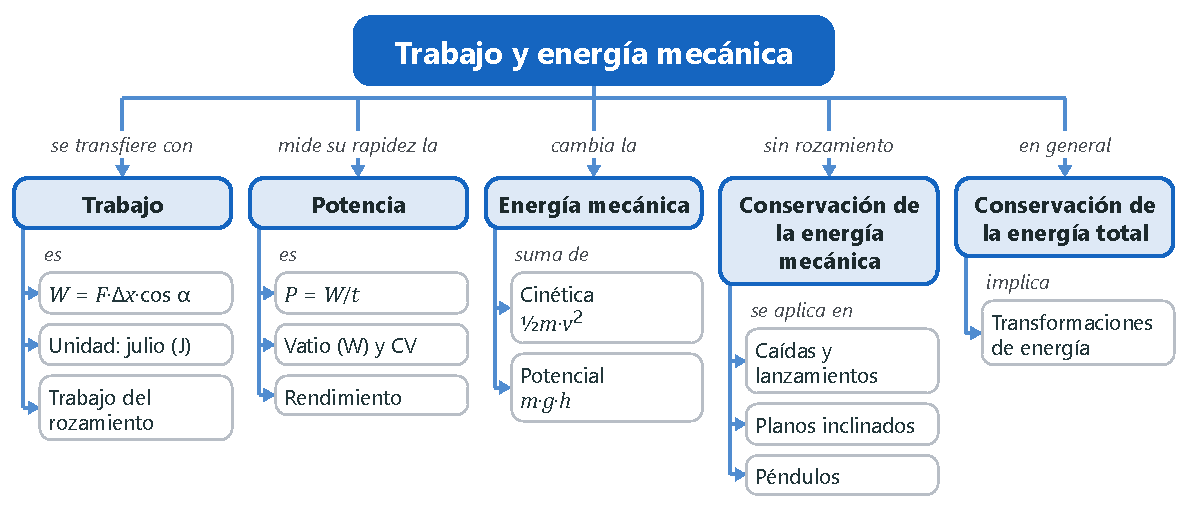
\includegraphics[width=\textwidth]{images/mapas_conceptuales/mapa_UD11}
\end{figure}

%========================================================================================
%\section*{Para empezar: el consumo de electricidad y de gas}
%\addcontentsline{toc}{section}{Para empezar: el consumo de electricidad y de gas}
%========================================================================================
%
%La electricidad nos proporciona energía para realizar trabajo: la usan todos los electrodomésticos y todos los aparatos con motores eléctricos. Las compañías venden la electricidad por «unidades», y esa unidad es el \textbf{kilovatio hora} (\unit{\kilo\watt\hour}). El contador de casa registra los kilovatios hora consumidos, y el precio depende del contrato con la comercializadora. Un electrodoméstico de gran potencia consume energía más deprisa, por lo que su funcionamiento resulta más caro que el de uno de menor potencia.
%
%Con el gas natural ocurre algo parecido. El contador mide el volumen de gas en metros cúbicos, pero en la factura el consumo aparece en kilovatios hora: no se paga por el volumen, sino por la \textbf{energía} que proporciona el gas al quemarse. Como el volumen de un gas cambia con la presión y la temperatura, y no todos los gases tienen la misma composición, cada compañía aplica un «factor de conversión»: cada metro cúbico de gas natural aporta unos \qty{11}{\kilo\watt\hour}. En el caso del gas butano, que se vende en bombonas de \qty{12.5}{\kg}, cada bombona proporciona unos \qty{159}{\kilo\watt\hour}.
%
%Consumir energía de forma eficiente y elegir fuentes renovables tiene que ver con el \textbf{ODS 7} (\emph{Energía asequible y no contaminante}), que busca aumentar el uso de energías renovables y mejorar la eficiencia energética, y con el \textbf{ODS 12} (\emph{Producción y consumo responsables}), que pide un uso eficiente de los recursos naturales.
%
%En esta unidad estudiaremos qué es el \textbf{trabajo} para la física, cómo se mide la rapidez con que se realiza (la \textbf{potencia}) y qué es la \textbf{energía mecánica}, y descubriremos una de las leyes más importantes de la naturaleza: la conservación de la energía.
%
%\begin{exercise}
%    Haz una lista de aparatos que usen electricidad, en casa y en el instituto. Anota la potencia de algunos de ellos (viene en la etiqueta), estima cuántas horas funcionan al día y calcula la energía diaria que consumen en \unit{\kilo\watt\hour}.
%    \begin{solu}
%        Respuesta libre. Ejemplos: iluminación, ordenador, frigorífico, lavadora, horno, microondas, calefacción\ldots{} La energía se calcula como \(E = P \cdot t\): por ejemplo, un microondas de \qty{800}{\watt} que funciona \qty{15}{\minute} al día consume \(\num{0.8} \cdot \num{0.25} = \textcolor{red}{\qty{0.2}{\kilo\watt\hour}}\) diarios; una lavadora consume entre \qty{0.5}{\kilo\watt\hour} y \qty{1.5}{\kilo\watt\hour} por lavado, según la temperatura del agua.
%    \end{solu}
%\end{exercise}
%
%\begin{exercise}
%    ¿Por qué cuesta más hacer funcionar un electrodoméstico de mayor potencia que otro del mismo tipo con menos potencia?
%    \begin{solu}
%        Porque un aparato de mayor potencia \textcolor{red}{consume más energía en el mismo tiempo}, y lo que se paga es la energía consumida (los \unit{\kilo\watt\hour}).
%    \end{solu}
%\end{exercise}
%
%\begin{exercise}
%    Si el contador mide el gas en \unit{\cubic\m}, ¿por qué en la factura se indica en \unit{\kilo\watt\hour}? ¿Aportan la misma energía todos los metros cúbicos de gas?
%    \begin{solu}
%        Porque el gas \textcolor{red}{no se paga por su volumen, sino por la energía que proporciona}. Un metro cúbico de gas no siempre aporta la misma energía: depende de la presión, de la temperatura y de la composición del gas, por eso la compañía aplica un factor de conversión.
%    \end{solu}
%\end{exercise}
%
%\begin{exercise}
%    Una bombona de butano de \qty{12.5}{\kg} proporciona unos \qty{159}{\kilo\watt\hour}. ¿Cuánta energía aporta cada kilogramo de butano, en \unit{\kilo\watt\hour} y en julios?
%    \begin{solu}
%        \(\dfrac{159}{\num{12.5}} = \textcolor{red}{\qty{12.7}{\kilo\watt\hour}}\) por kilogramo, es decir, \(\num{12.7} \cdot \num{3.6e6} = \textcolor{red}{\qty{4.6e7}{\joule}}\).
%    \end{solu}
%\end{exercise}

%========================================================================================
\section{Trabajo y energía}
%========================================================================================

¿Estás haciendo trabajo mientras esperas el autobús con la mochila a la espalda? Si respondes que sí, estás confundiendo el esfuerzo muscular con el trabajo. Al sostener la mochila sin moverte te cansas, pero para la física no realizas ningún trabajo, porque no hay desplazamiento.

\begin{definition}[Trabajo]
    En física, decimos que una fuerza realiza un \textbf{trabajo} cuando produce un \textbf{desplazamiento} en la dirección de la fuerza.
\end{definition}

Un coche que se ha quedado sin gasolina en lo alto de una cuesta parece que no tiene energía. Sin embargo, si se suelta el freno, rodará cuesta abajo: tiene energía por estar a cierta altura.

\begin{definition}[Energía]
    La \textbf{energía} es la capacidad que tienen los cuerpos de producir transformaciones, por ejemplo, de realizar un trabajo.
\end{definition}

El trabajo y la energía son \textbf{magnitudes escalares}: quedan definidas con un número y su unidad, que en el SI es el \textbf{julio} (\unit{\joule}). De hecho, el trabajo es una forma de medir la energía que se transfiere de un cuerpo a otro.

\subsection{¿Cuándo realiza trabajo una fuerza?}

\begin{itemize}
    \item \textbf{Sin desplazamiento no hay trabajo.} Al empujar una pared, los músculos ejercen una fuerza, pero la pared no se mueve: no se realiza trabajo.
    \item \textbf{El desplazamiento debe producirse en la dirección de la fuerza.} Si llevamos una caja en brazos por un pasillo horizontal, la fuerza que hacemos para sostenerla es vertical y el desplazamiento es horizontal: esa fuerza no realiza trabajo.
\end{itemize}

\begin{figure}[H]
    \centering
    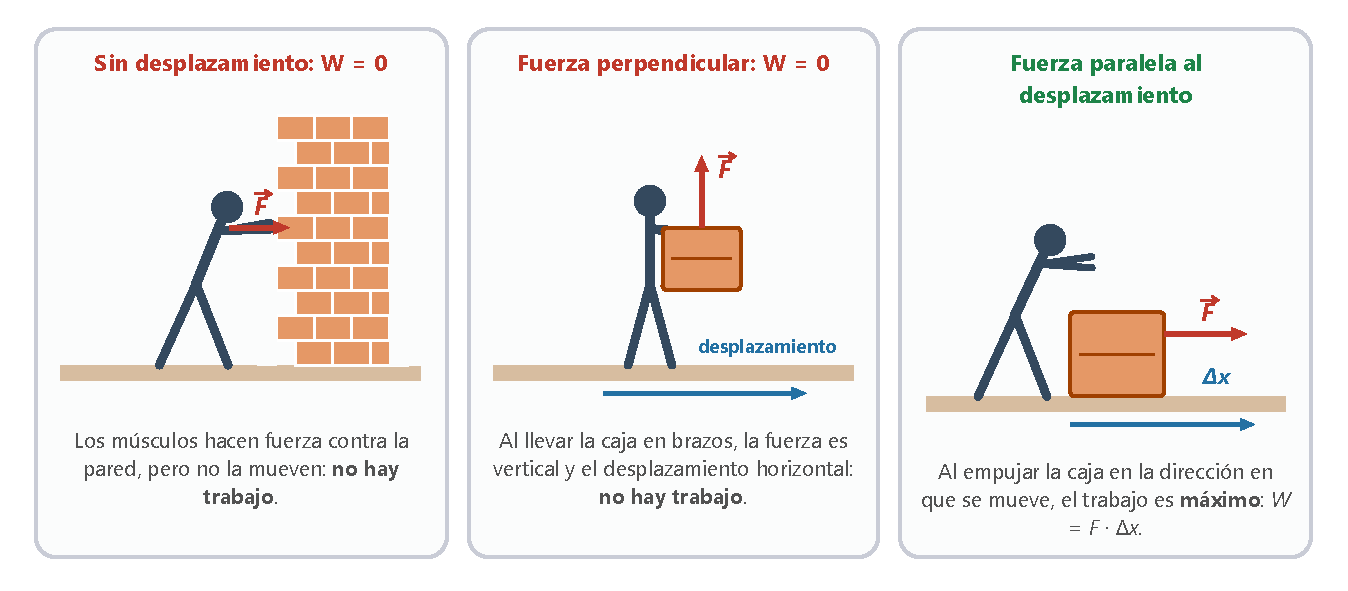
\includegraphics[width=\textwidth]{images/UD11/trabajo_casos}
    \caption{Solo hay trabajo si la fuerza produce un desplazamiento en su dirección.}
    \label{fig:trabajo_casos}
\end{figure}

\begin{exercise}
    ¿Realizas trabajo al levantar la mochila desde el suelo hasta la altura a la que la sostienes? ¿Y al subir una escalera con la mochila a cuestas?
    \begin{solu}
        \textcolor{red}{Sí en los dos casos}: ejerces una fuerza vertical, hacia arriba, para vencer el peso de la mochila, y la mochila se desplaza en esa misma dirección (sube).
    \end{solu}
\end{exercise}

\begin{exercise}
    Responde verdadero o falso y justifica tu respuesta:
    \begin{enumerate}[label=\alph*)]
        \item Siempre que hacemos un esfuerzo muscular se realiza trabajo.
        \item Nuestros brazos realizan trabajo al llevar la bolsa de la compra desde el supermercado hasta casa por una calle horizontal.
        \item La energía es la capacidad que tienen los cuerpos de realizar un trabajo.
        \item Realizamos un trabajo cuando empujamos fuertemente una pared.
    \end{enumerate}
    \begin{solu}
        a) \textcolor{red}{Falso}: si no hay desplazamiento, no hay trabajo. b) \textcolor{red}{Falso}: la fuerza de los brazos es vertical y el desplazamiento horizontal. c) \textcolor{red}{Verdadero}. d) \textcolor{red}{Falso}: la pared no se desplaza.
    \end{solu}
\end{exercise}

\subsection*{Actividades de consolidación: trabajo y energía}

\begin{exercise}
    ¿Coincide el significado de la palabra \emph{trabajo} en el lenguaje cotidiano y en física?
    \begin{solu}
        \textcolor{red}{No}. En el lenguaje cotidiano el trabajo se relaciona con el esfuerzo o el cansancio, haya o no desplazamiento; en física solo hay trabajo si una \textcolor{red}{fuerza produce un desplazamiento} en su dirección.
    \end{solu}
\end{exercise}

\begin{exercise}
    ¿Realizas trabajo, en el sentido físico, mientras resuelves estas cuestiones en clase?
    \begin{solu}
        Prácticamente \textcolor{red}{no}: aunque pensar cansa, no ejerces ninguna fuerza que desplace un cuerpo (salvo el pequeño trabajo de mover el bolígrafo).
    \end{solu}
\end{exercise}

\begin{exercise}
    Explica si realizas trabajo o no cuando:
    \begin{enumerate}[label=\alph*)]
        \item Levantas una maleta desde el suelo.
        \item Esperas el tren en el andén con la maleta en la mano.
        \item Subes las escaleras con la maleta.
        \item Empujas con fuerza la pared de tu habitación.
    \end{enumerate}
    \begin{solu}
        a) \textcolor{red}{Sí}: la fuerza y el desplazamiento son verticales. b) \textcolor{red}{No}: no hay desplazamiento. c) \textcolor{red}{Sí}: la maleta sube en la dirección de la fuerza. d) \textcolor{red}{No}: la pared no se desplaza.
    \end{solu}
\end{exercise}

\begin{exercise}
    Indica en cuáles de estas situaciones se realiza trabajo y en cuáles no: a) una persona empuja un mueble y lo desplaza por el suelo; b) un alumno camina por un pasillo con la mochila a la espalda; c) una persona levanta del suelo una bolsa de la compra; d) una persona está quieta sosteniendo una bolsa.
    \begin{solu}
        Se realiza trabajo en \textcolor{red}{a) y c)}. En b) la fuerza que sostiene la mochila es perpendicular al desplazamiento, y en d) no hay desplazamiento.
    \end{solu}
\end{exercise}

%========================================================================================
\section{Trabajo realizado por una fuerza constante}
%========================================================================================

Cuando una fuerza constante tiene la misma dirección y sentido que el desplazamiento que produce, el trabajo es el producto de la fuerza por el desplazamiento:
\[ \text{trabajo} = \text{fuerza} \times \text{desplazamiento} \qquad W = F \cdot \Delta x \]
donde \(W\) es el trabajo, \(F\) es la fuerza (constante) y \(\Delta x\) el desplazamiento producido en la dirección de la fuerza.

En una gráfica fuerza-desplazamiento, una fuerza constante es una recta horizontal, y el trabajo que realiza es el \textbf{área del rectángulo} que queda bajo ella: base (\(\Delta x\)) por altura (\(F\)).

\begin{center}
    \begin{tikzpicture}
        \begin{axis}[grafica, width=8cm, height=5cm, xlabel={\(x\) (m)}, ylabel={\(F\) (N)}, xmin=0, xmax=4.5, ymin=0, ymax=7.5, title={\small \(W = F \cdot \Delta x = 6 \cdot \num{2.5} = \qty{15}{\joule}\) (área del rectángulo)}]
            \addplot[mark=none, fill=yellow!60, draw=red!75!black, line width=1.4pt] coordinates {(0,0) (0,6) (2.5,6) (2.5,0)};
            \node at (axis cs:1.25,3) {\(W\)};
        \end{axis}
    \end{tikzpicture}
\end{center}

\subsection{¿En qué unidad se expresa el trabajo?}

En el SI, el trabajo se mide en \textbf{julios} (\unit{\joule}). Un julio es el trabajo que realiza una fuerza de un newton al desplazar su punto de aplicación un metro en su misma dirección:
\[ \qty{1}{\joule} = \qty{1}{\newton} \cdot \qty{1}{\m} \]
Su ecuación de dimensiones es \([W] = \mathrm{M \cdot L^2 \cdot T^{-2}}\).

\subsection{¿Qué sucede si la fuerza tiene la dirección y el sentido del desplazamiento?}

Entonces el trabajo es \textbf{máximo y positivo}: \(W = F \cdot \Delta x\). Cuando empujamos un baúl en la misma dirección en la que queremos moverlo, aprovechamos toda la fuerza.

\begin{example}
    Calcula el trabajo que realizas al subir una mochila de \qty{8}{\kg} hasta una altura de \qty{1.5}{\m}.

    Para subirla hay que ejercer una fuerza igual a su peso: \(F = m \cdot g = 8 \cdot \num{9.8} = \qty{78.4}{\newton}\). Como la fuerza y el desplazamiento son verticales y hacia arriba:
    \[ W = F \cdot \Delta x = \num{78.4} \cdot \num{1.5} = \textcolor{red}{\qty{117.6}{\joule}} \]
\end{example}

\subsection{¿Qué sucede si la fuerza es perpendicular al desplazamiento?}

El trabajo realizado por esa fuerza es \textbf{nulo}: \(W = 0\). Si llevamos el baúl en brazos de un sitio a otro por un suelo horizontal, la fuerza que hacemos es vertical y el desplazamiento horizontal: no realizamos trabajo (figura~\ref{fig:trabajo_casos}).

\subsection{¿Realiza trabajo la fuerza de rozamiento?}

Sí, pero su trabajo es \textbf{negativo}, porque la fuerza de rozamiento tiene sentido contrario al desplazamiento (figura~\ref{fig:trabajo_angulo}):
\[ W_{\text{roz}} = -F_{\text{roz}} \cdot \Delta x \]
Recuerda que, en una superficie horizontal, \(F_{\text{roz}} = \mu \cdot m \cdot g\), donde \(\mu\) es el coeficiente de rozamiento.

\begin{example}
    Arrastras una mochila de \qty{10}{\kg} \qty{2}{\m} por un suelo horizontal. Si el coeficiente de rozamiento es \(\mu = \num{0.1}\), ¿qué trabajo realiza la fuerza de rozamiento?
    \[ W_{\text{roz}} = -\mu \cdot m \cdot g \cdot \Delta x = -\num{0.1} \cdot 10 \cdot \num{9.8} \cdot 2 = \textcolor{red}{\qty{-19.6}{\joule}} \]
\end{example}

\subsection{¿Y si la fuerza forma un ángulo con el desplazamiento?}

Cuando la fuerza forma un ángulo \(\theta\) con el desplazamiento, \textbf{solo realiza trabajo la componente de la fuerza en la dirección del desplazamiento}, \(F_x = F \cdot \cos\theta\) (figura~\ref{fig:trabajo_angulo}). Por tanto:
\[ W = F_x \cdot \Delta x = F \cdot \Delta x \cdot \cos\theta \]
Esta expresión incluye los casos anteriores: si \(\theta = \ang{0}\), \(\cos\theta = 1\) y el trabajo es máximo; si \(\theta = \ang{90}\), \(\cos\theta = 0\) y el trabajo es nulo; si \(\theta = \ang{180}\) (como el rozamiento), \(\cos\theta = -1\) y el trabajo es negativo.

\begin{figure}[H]
    \centering
    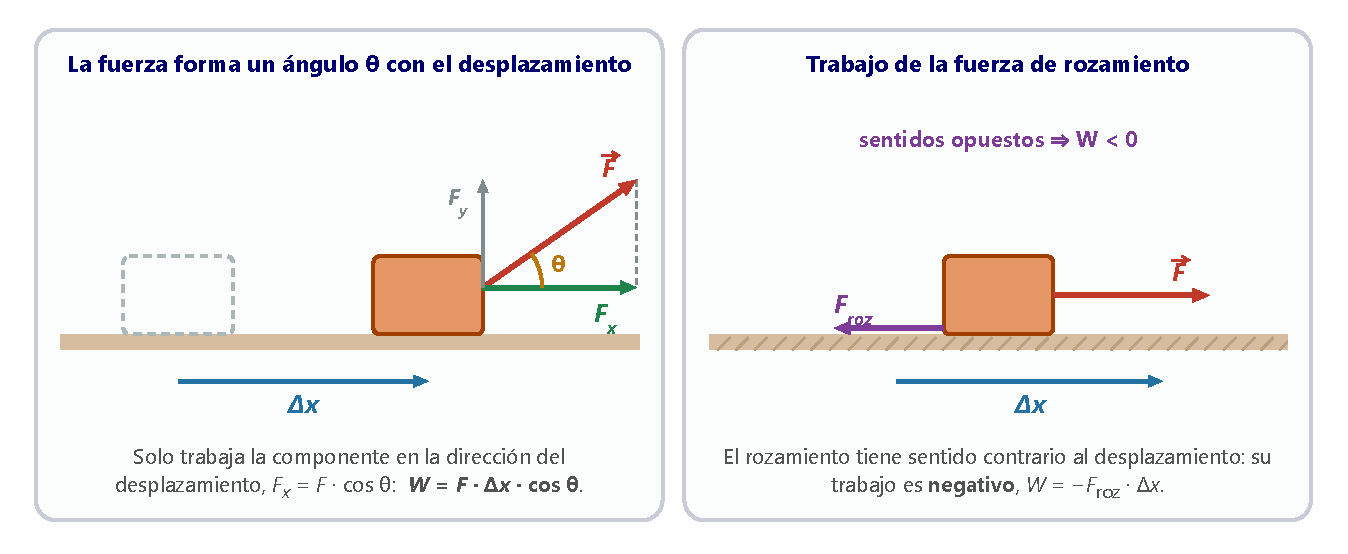
\includegraphics[width=\textwidth]{images/UD11/trabajo_angulo}
    \caption{Trabajo de una fuerza que forma un ángulo con el desplazamiento y de la fuerza de rozamiento.}
    \label{fig:trabajo_angulo}
\end{figure}

\begin{example}
    Arrastras una mochila \qty{2}{\m} por un suelo sin rozamiento tirando de ella con una fuerza de \qty{50}{\newton} que forma un ángulo de \ang{60} con la horizontal. ¿Qué trabajo realizas?
    \[ W = F \cdot \Delta x \cdot \cos\theta = 50 \cdot 2 \cdot \cos\ang{60} = 50 \cdot 2 \cdot \num{0.5} = \textcolor{red}{\qty{50}{\joule}} \]
    Solo se aprovecha la mitad de la fuerza: la componente vertical no realiza trabajo.
\end{example}

\begin{exercise}
    Escribe la ecuación de dimensiones del trabajo.
    \begin{solu}
        \([W] = [F] \cdot [\Delta x] = \mathrm{M \cdot L \cdot T^{-2}} \cdot \mathrm{L} = \textcolor{red}{\mathrm{M \cdot L^2 \cdot T^{-2}}}\).
    \end{solu}
\end{exercise}

\begin{exercise}
    En esta gráfica se representa una fuerza en función del desplazamiento que produce. ¿Cuánto vale la fuerza? ¿Qué desplazamiento produce? Calcula el trabajo que realiza.
    \begin{center}
        \begin{tikzpicture}
            \begin{axis}[grafica, width=6.5cm, height=4.2cm, xlabel={\(x\) (m)}, ylabel={\(F\) (N)}, xmin=0, xmax=5, ymin=0, ymax=10, ytick={0,2,...,10}]
                \addplot[mark=none, fill=yellow!60, draw=red!75!black, line width=1.4pt] coordinates {(0,0) (0,8) (4,8) (4,0)};
            \end{axis}
        \end{tikzpicture}
    \end{center}
    \begin{solu}
        La fuerza vale \textcolor{red}{\qty{8}{\newton}} y produce un desplazamiento de \textcolor{red}{\qty{4}{\m}}. El trabajo es el área del rectángulo: \(W = 8 \cdot 4 = \textcolor{red}{\qty{32}{\joule}}\).
    \end{solu}
\end{exercise}

\begin{exercise}
    ¿Puede ser nulo el trabajo de una fuerza aunque ni la fuerza ni el desplazamiento sean nulos?
    \begin{solu}
        \textcolor{red}{Sí}, cuando la fuerza es \textcolor{red}{perpendicular} al desplazamiento (\(\cos\ang{90} = 0\)).
    \end{solu}
\end{exercise}

\begin{exercise}
    Calcula el trabajo que realizas al arrastrar un baúl \qty{5}{\m} por un suelo horizontal sin rozamiento aplicando una fuerza de \qty{50}{\newton} que forma un ángulo de \ang{30} con la horizontal.
    \begin{solu}
        \(W = F \cdot \Delta x \cdot \cos\theta = 50 \cdot 5 \cdot \cos\ang{30} = 250 \cdot \num{0.866} = \textcolor{red}{\qty{216.5}{\joule}}\).
    \end{solu}
\end{exercise}

\begin{exercise}
    Una operaria arrastra un fardo \qty{10}{\m} por el suelo, sin rozamiento, con un cable que forma un ángulo de \ang{45} con la horizontal. Si el trabajo realizado es de \qty{1273}{\joule}, ¿qué fuerza ha aplicado?
    \begin{solu}
        \(F = \dfrac{W}{\Delta x \cdot \cos\theta} = \dfrac{1273}{10 \cdot \cos\ang{45}} = \dfrac{1273}{\num{7.07}} = \textcolor{red}{\qty{180}{\newton}}\).
    \end{solu}
\end{exercise}

\begin{exercise}
    Un reponedor arrastra un fardo de \qty{50}{\kg} una distancia de \qty{5}{\m} por una superficie horizontal sin rozamiento, tirando de un cable que forma \ang{30} con la horizontal. ¿Qué trabajo realiza si la fuerza que aplica es igual al peso del fardo?
    \begin{solu}
        \(F = 50 \cdot \num{9.8} = \qty{490}{\newton}\); \(W = 490 \cdot 5 \cdot \cos\ang{30} = \textcolor{red}{\qty{2122}{\joule}}\).
    \end{solu}
\end{exercise}

\subsection*{Actividades de consolidación: trabajo de una fuerza constante}

\begin{exercise}
    De la expresión del trabajo, \(W = F \cdot \Delta x\), se deduce también que \(F = W/\Delta x\) y \(\Delta x = W/F\). Úsalas para completar la tabla en tu cuaderno:
    \begin{center}
        % --- tabla antigua ---
        % \begin{tblr}{colspec={ccc}, hlines, vlines, row{1}={bg=ocre!85, fg=white, font=\bfseries}}
            % Fuerza (N) & Desplazamiento (m) & Trabajo (J) \\
            % 200 & \num{2.00} & \ldots \\
            % \ldots & \num{5.00} & 500 \\
            % 50 & \ldots & 100 \\
        % \end{tblr}
        % --- tabla nueva ---
        \begin{tabular}{@{}ccc@{}}
            \toprule
            \textbf{Fuerza (N)} & \textbf{Desplazamiento (m)} & \textbf{Trabajo (J)} \\
            \midrule
            200 & \num{2.00} & \ldots \\[3pt]
            \ldots & \num{5.00} & 500 \\[3pt]
            50 & \ldots & 100 \\
            \bottomrule
        \end{tabular}
    \end{center}
    \begin{solu}
        \(W = 200 \cdot 2 = \textcolor{red}{\qty{400}{\joule}}\); \(F = \dfrac{500}{5} = \textcolor{red}{\qty{100}{\newton}}\); \(\Delta x = \dfrac{100}{50} = \textcolor{red}{\qty{2}{\m}}\).
    \end{solu}
\end{exercise}

\begin{exercise}
    ¿Qué trabajo realizas al subir un paquete de \qty{4.5}{\kg} desde el suelo hasta una mesa de \qty{90}{\cm} de altura? ¿Y al llevarlo después en brazos por el pasillo de tu casa?
    \begin{solu}
        Subirlo: \(W = m \cdot g \cdot h = \num{4.5} \cdot \num{9.8} \cdot \num{0.9} = \textcolor{red}{\qty{39.7}{\joule}}\). Por el pasillo: \textcolor{red}{\qty{0}{\joule}}, porque la fuerza que hacemos (vertical) es perpendicular al desplazamiento (horizontal).
    \end{solu}
\end{exercise}

\begin{exercise}
    ¿Qué trabajo se realiza cuando una fuerza desplaza su punto de aplicación, en su misma dirección: a) \qty{3.0}{\m}, si la fuerza es de \qty{6}{\newton}; b) \qty{0.5}{\m}, si es de \qty{12}{\newton}; c) \qty{10}{\mm}, si es de \qty{10}{\newton}?
    \begin{solu}
        a) \(6 \cdot 3 = \textcolor{red}{\qty{18}{\joule}}\); b) \(12 \cdot \num{0.5} = \textcolor{red}{\qty{6}{\joule}}\); c) \(10 \cdot \num{0.010} = \textcolor{red}{\qty{0.1}{\joule}}\).
    \end{solu}
\end{exercise}

\begin{exercise}
    Una fuerza constante de \qty{9}{\newton} desplaza su punto de aplicación \qty{6}{\m} en su misma dirección. Dibuja la gráfica \(F\)--\(x\) y calcula el trabajo a partir de ella.
    \begin{solu}
        La gráfica es una recta horizontal a la altura \(F = \qty{9}{\newton}\) entre \(x = 0\) y \(x = \qty{6}{\m}\). El trabajo es el área del rectángulo: \(W = 9 \cdot 6 = \textcolor{red}{\qty{54}{\joule}}\).
    \end{solu}
\end{exercise}

\begin{exercise}
    Calcula el trabajo que realiza la fuerza de rozamiento cuando se arrastra una maleta de \qty{40}{\kg} \qty{5}{\m} sobre un suelo horizontal, si el coeficiente de rozamiento es \num{0.1}.
    \begin{solu}
        \(W_{\text{roz}} = -\mu \cdot m \cdot g \cdot \Delta x = -\num{0.1} \cdot 40 \cdot \num{9.8} \cdot 5 = \textcolor{red}{\qty{-196}{\joule}}\).
    \end{solu}
\end{exercise}

\begin{exercise}
    Arrastras un baúl de \qty{14}{\kg} \qty{4}{\m} por un suelo horizontal con un coeficiente de rozamiento de \num{0.1}. ¿Qué trabajo realiza la fuerza de rozamiento?
    \begin{solu}
        \(W_{\text{roz}} = -\num{0.1} \cdot 14 \cdot \num{9.8} \cdot 4 = \textcolor{red}{\qty{-54.9}{\joule}}\).
    \end{solu}
\end{exercise}

\begin{exercise}
    Una persona arrastra una caja de \qty{10}{\kg} \qty{10}{\m} por un suelo horizontal tirando con una fuerza constante de \qty{100}{\newton} que forma \ang{40} con la horizontal. La fuerza de rozamiento es de \qty{50}{\newton}. Calcula el trabajo realizado: a) por la fuerza de \qty{100}{\newton}; b) por el rozamiento; c) en total (trabajo neto).
    \begin{solu}
        a) \(W = 100 \cdot 10 \cdot \cos\ang{40} = \textcolor{red}{\qty{766}{\joule}}\). b) \(W_{\text{roz}} = -50 \cdot 10 = \textcolor{red}{\qty{-500}{\joule}}\). c) \(W_{\text{neto}} = 766 - 500 = \textcolor{red}{\qty{266}{\joule}}\). (El peso y la normal no realizan trabajo, porque son perpendiculares al desplazamiento.)
    \end{solu}
\end{exercise}

\begin{exercise}
    Una fuerza constante de \qty{25}{\newton} actúa sobre un cuerpo de \qty{10}{\kg} que se desplaza \qty{10}{\m} por un plano horizontal, en la dirección de la fuerza. Si el coeficiente de rozamiento es \num{0.1}, calcula el trabajo: a) de la fuerza aplicada; b) de la fuerza de rozamiento; c) total.
    \begin{solu}
        a) \(W = 25 \cdot 10 = \textcolor{red}{\qty{250}{\joule}}\). b) \(W_{\text{roz}} = -\num{0.1} \cdot 10 \cdot \num{9.8} \cdot 10 = \textcolor{red}{\qty{-98}{\joule}}\). c) \(W_{\text{total}} = 250 - 98 = \textcolor{red}{\qty{152}{\joule}}\).
    \end{solu}
\end{exercise}

%========================================================================================
\section[La potencia]{Relación trabajo-tiempo: la potencia}
%========================================================================================

Cuando subes unas escaleras corriendo, haces el mismo trabajo que cuando las subes despacio (elevas tu peso la misma altura), pero lo haces en menos tiempo: desarrollas más \textbf{potencia}.

\begin{definition}[Potencia]
    La \textbf{potencia}, \(P\), es la magnitud que mide la rapidez con la que se realiza un trabajo:
    \[ \text{potencia} = \frac{\text{trabajo realizado}}{\text{tiempo empleado}} \qquad P = \frac{W}{t} \]
    Su unidad en el SI es el \textbf{vatio} (\unit{\watt}): la potencia de una máquina que realiza un trabajo de \qty{1}{\joule} en \qty{1}{\s}. \(\qty{1}{\watt} = \qty{1}{\joule\per\s}\); \(\qty{1}{\kilo\watt} = \qty{1000}{\watt}\).
\end{definition}

\subsection{Potencia teórica y potencia real: el rendimiento}

En la práctica, la potencia real (útil) de una máquina es menor que su potencia teórica, debido a los rozamientos, las vibraciones y los calentamientos de sus piezas. Para medir esta pérdida se define el \textbf{rendimiento}:
\[ \text{rendimiento} = \frac{\text{potencia real}}{\text{potencia teórica}} \cdot 100 = \frac{\text{trabajo útil}}{\text{trabajo realizado}} \cdot 100 \]
El rendimiento de una máquina se expresa en porcentaje y \textbf{siempre es menor del \qty{100}{\percent}}.

\begin{example}
    El motor de un montacargas tiene una potencia teórica de \qty{1450}{\watt} y tarda \qty{14}{\s} en subir un bloque de \qty{100}{\kg} hasta \qty{16}{\m} de altura. Calcula su potencia real y su rendimiento.

    El trabajo útil es el necesario para subir el bloque: \(W = m \cdot g \cdot h = 100 \cdot \num{9.8} \cdot 16 = \qty{15680}{\joule}\).
    \[ P_{\text{real}} = \frac{W}{t} = \frac{15680}{14} = \textcolor{red}{\qty{1120}{\watt}} \qquad \text{rendimiento} = \frac{1120}{1450} \cdot 100 = \textcolor{red}{\qty{77}{\percent}} \]
\end{example}

\subsection{Otras unidades de trabajo y de potencia}

\begin{itemize}
    \item Las compañías eléctricas miden la energía consumida en \textbf{kilovatios hora} (\unit{\kilo\watt\hour}): el trabajo que realiza una máquina de \qty{1}{\kilo\watt} funcionando durante una hora.
    \[ \qty{1}{\kilo\watt\hour} = \qty{1000}{\watt} \cdot \qty{3600}{\s} = \qty{3.6e6}{\joule} \]
    \item En física de partículas se usa el \textbf{electronvoltio} (\unit{\electronvolt}): \(\qty{1}{\electronvolt} = \qty{1.6e-19}{\joule}\). Sus múltiplos son el \unit{\mega\electronvolt} (\qty{e6}{\electronvolt}), el \unit{\giga\electronvolt} (\qty{e9}{\electronvolt}) y el \unit{\tera\electronvolt} (\qty{e12}{\electronvolt}).
    \item El escocés \textbf{James Watt} (1736-1819), que perfeccionó la máquina de vapor, definió para venderla a los dueños de minas el \textbf{caballo de vapor} (\unit{\CV}), la potencia de una máquina capaz de sustituir a un caballo: \(\qty{1}{\CV} = \qty{736}{\watt}\). Todavía se usa para la potencia de los coches.
\end{itemize}

\begin{exercise}
    Escribe la ecuación de dimensiones de la potencia.
    \begin{solu}
        \([P] = \dfrac{[W]}{[t]} = \dfrac{\mathrm{M \cdot L^2 \cdot T^{-2}}}{\mathrm{T}} = \textcolor{red}{\mathrm{M \cdot L^2 \cdot T^{-3}}}\).
    \end{solu}
\end{exercise}

\begin{exercise}
    Dos máquinas realizan el mismo trabajo en tiempos distintos. ¿Cuál tiene más potencia?
    \begin{solu}
        La que lo realiza \textcolor{red}{en menos tiempo}.
    \end{solu}
\end{exercise}

\begin{exercise}
    El motor de una lavadora tiene una potencia teórica de \qty{2000}{\watt} y un rendimiento del \qty{75}{\percent}. a) ¿Cuál es su potencia real? b) ¿Qué trabajo útil realiza en \qty{45}{\minute}?
    \begin{solu}
        a) \(P_{\text{real}} = \num{0.75} \cdot 2000 = \textcolor{red}{\qty{1500}{\watt}}\). b) \(W = P \cdot t = 1500 \cdot (45 \cdot 60) = \textcolor{red}{\qty{4.05e6}{\joule}}\).
    \end{solu}
\end{exercise}

\begin{exercise}
    Expresa en kilovatios hora: a) \qty{9e6}{\joule}; b) \qty{7.2e6}{\joule}; c) \qty{1.8e7}{\joule}.
    \begin{solu}
        Se divide entre \num{3.6e6}: a) \textcolor{red}{\qty{2.5}{\kilo\watt\hour}}; b) \textcolor{red}{\qty{2}{\kilo\watt\hour}}; c) \textcolor{red}{\qty{5}{\kilo\watt\hour}}.
    \end{solu}
\end{exercise}

\begin{exercise}
    Calcula la potencia de una máquina que realiza un trabajo de \qty{2e4}{\joule} en \qty{1}{\minute}.
    \begin{solu}
        \(P = \dfrac{W}{t} = \dfrac{\num{2e4}}{60} = \textcolor{red}{\qty{333}{\watt}}\).
    \end{solu}
\end{exercise}

\begin{exercise}
    Expresa en julios: a) \qty{2.5}{\kilo\watt\hour}; b) \qty{10}{\electronvolt}; c) \qty{5}{\mega\electronvolt}; d) \qty{3}{\giga\electronvolt}.
    \begin{solu}
        a) \(\num{2.5} \cdot \num{3.6e6} = \textcolor{red}{\qty{9e6}{\joule}}\); b) \(10 \cdot \num{1.6e-19} = \textcolor{red}{\qty{1.6e-18}{\joule}}\); c) \(\num{5e6} \cdot \num{1.6e-19} = \textcolor{red}{\qty{8e-13}{\joule}}\); d) \(\num{3e9} \cdot \num{1.6e-19} = \textcolor{red}{\qty{4.8e-10}{\joule}}\).
    \end{solu}
\end{exercise}

\subsection*{Actividades de consolidación: la potencia}

\begin{exercise}
    Una máquina realiza un trabajo de \qty{2000}{\joule} con un rendimiento del \qty{25}{\percent}. ¿Qué trabajo útil se obtiene realmente?
    \begin{solu}
        \(W_{\text{útil}} = \num{0.25} \cdot 2000 = \textcolor{red}{\qty{500}{\joule}}\).
    \end{solu}
\end{exercise}

\begin{exercise}
    Para calcular su potencia muscular, una atleta de \qty{60}{\kg} sube corriendo un tramo de escaleras de \qty{10}{\m} de altura y tarda \qty{12}{\s}. ¿Qué potencia desarrolla?
    \begin{solu}
        \(P = \dfrac{m \cdot g \cdot h}{t} = \dfrac{60 \cdot \num{9.8} \cdot 10}{12} = \textcolor{red}{\qty{490}{\watt}}\).
    \end{solu}
\end{exercise}

\begin{exercise}
    Un gato de \qty{50}{\newton} de peso trepa a un árbol de \qty{3}{\m} en \qty{2}{\s}. ¿Qué trabajo realiza? ¿Qué potencia desarrolla?
    \begin{solu}
        \(W = 50 \cdot 3 = \textcolor{red}{\qty{150}{\joule}}\); \(P = \dfrac{150}{2} = \textcolor{red}{\qty{75}{\watt}}\).
    \end{solu}
\end{exercise}

\begin{exercise}
    ¿Qué potencia tiene una máquina que sube una masa de \qty{100}{\kg} a \qty{20}{\m} de altura en \qty{15}{\s}?
    \begin{solu}
        \(W = 100 \cdot \num{9.8} \cdot 20 = \qty{19600}{\joule}\); \(P = \dfrac{19600}{15} = \textcolor{red}{\qty{1307}{\watt}}\).
    \end{solu}
\end{exercise}

\begin{exercise}
    Un motor realiza un trabajo de \qty{1500}{\joule} en \qty{10}{\s}. a) ¿Cuál es su potencia? b) ¿Cuánto tardaría en hacer ese trabajo una máquina de \qty{15}{\watt}?
    \begin{solu}
        a) \(P = \dfrac{1500}{10} = \textcolor{red}{\qty{150}{\watt}}\). b) \(t = \dfrac{W}{P} = \dfrac{1500}{15} = \textcolor{red}{\qty{100}{\s}}\).
    \end{solu}
\end{exercise}

\begin{exercise}
    ¿Cuántos kilovatios hora se consumen cuando: a) una estufa de \qty{2500}{\watt} está encendida dos horas; b) una lavadora de \qty{2000}{\watt} funciona una hora y media?
    \begin{solu}
        a) \(E = P \cdot t = \num{2.5} \cdot 2 = \textcolor{red}{\qty{5}{\kilo\watt\hour}}\). b) \(E = 2 \cdot \num{1.5} = \textcolor{red}{\qty{3}{\kilo\watt\hour}}\).
    \end{solu}
\end{exercise}

\begin{exercise}
    La energía de un electrón en un acelerador de partículas es de \qty{3}{\mega\electronvolt}. Exprésala en julios.
    \begin{solu}
        \(E = \num{3e6} \cdot \num{1.6e-19} = \textcolor{red}{\qty{4.8e-13}{\joule}}\).
    \end{solu}
\end{exercise}

\begin{exercise}
    Tres grúas suben un paquete de ladrillos de \qty{500}{\kg}: la grúa A lo eleva \qty{20}{\m} en \qty{15}{\s}; la B, \qty{15}{\m} en \qty{10}{\s}; y la C, \qty{10}{\m} en \qty{5}{\s}. ¿Cuál desarrolla más potencia?
    \begin{solu}
        \(P_A = \dfrac{500 \cdot \num{9.8} \cdot 20}{15} = \qty{6533}{\watt}\); \(P_B = \dfrac{500 \cdot \num{9.8} \cdot 15}{10} = \qty{7350}{\watt}\); \(P_C = \dfrac{500 \cdot \num{9.8} \cdot 10}{5} = \qty{9800}{\watt}\).
        La \textcolor{red}{grúa C} es la más potente.
    \end{solu}
\end{exercise}

\begin{exercise}
    ¿Cuál de estas máquinas tiene mayor rendimiento? Máquina A: potencia real \qty{300}{\watt} y potencia teórica \qty{750}{\watt}. Máquina B: trabajo útil \qty{2275}{\joule} y trabajo realizado \qty{6500}{\joule}.
    \begin{solu}
        A: \(\dfrac{300}{750} \cdot 100 = \qty{40}{\percent}\); B: \(\dfrac{2275}{6500} \cdot 100 = \qty{35}{\percent}\). Tiene más rendimiento la \textcolor{red}{máquina A}.
    \end{solu}
\end{exercise}

\begin{exercise}
    El motor de un elevador sube un bloque de \qty{500}{\kg} hasta \qty{15}{\m} de altura en \qty{20}{\s}. a) ¿Qué trabajo realiza? b) ¿Cuál es su potencia? c) Si su potencia teórica es de \qty{5000}{\watt}, ¿cuál es su rendimiento?
    \begin{solu}
        a) \(W = 500 \cdot \num{9.8} \cdot 15 = \textcolor{red}{\qty{73500}{\joule}}\). b) \(P = \dfrac{73500}{20} = \textcolor{red}{\qty{3675}{\watt}}\). c) \(\dfrac{3675}{5000} \cdot 100 = \textcolor{red}{\qty{73.5}{\percent}}\).
    \end{solu}
\end{exercise}

\begin{exercise}
    ¿Cuánto tiempo debe funcionar una máquina de \qty{100}{\watt} para realizar el mismo trabajo que otra de \qty{20}{\CV} en media hora?
    \begin{solu}
        \(P = 20 \cdot 736 = \qty{14720}{\watt}\); \(W = 14720 \cdot 1800 = \qty{2.65e7}{\joule}\).
        \(t = \dfrac{W}{P} = \dfrac{\num{2.65e7}}{100} = \qty{2.65e5}{\s} = \textcolor{red}{\qty{73.6}{\hour}}\) (más de tres días).
    \end{solu}
\end{exercise}

\begin{exercise}
    Una escaladora de \qty{50}{\kg} sube una pared de \qty{10}{\m} en \qty{40}{\s}. Calcula: a) su peso; b) el trabajo realizado; c) su potencia.
    \begin{solu}
        a) \(P = 50 \cdot \num{9.8} = \textcolor{red}{\qty{490}{\newton}}\). b) \(W = 490 \cdot 10 = \textcolor{red}{\qty{4900}{\joule}}\). c) \(P = \dfrac{4900}{40} = \textcolor{red}{\qty{122.5}{\watt}}\).
    \end{solu}
\end{exercise}

%========================================================================================
\section{Energía mecánica}
%========================================================================================

Un cuerpo posee energía cuando tiene capacidad para realizar un trabajo. A su vez, el trabajo es la forma de medir la cantidad de energía que se transfiere de un cuerpo a otro o que pasa de una forma a otra. La \textbf{energía mecánica} se presenta en dos formas: la \textbf{cinética}, asociada al movimiento, y la \textbf{potencial}, asociada a la posición.

\subsection{Energía cinética}

Supongamos que aplicamos una fuerza constante, \(F\), a un cuerpo de masa \(m\) que está en reposo (figura~\ref{fig:energia_cinetica}). El cuerpo se acelera y, al cabo de un tiempo \(t\), ha recorrido una distancia \(\Delta x\) y tiene una velocidad \(v\). Como la aceleración es constante, \(a = v/t\), y:
\[ F = m \cdot a = m \cdot \frac{v}{t} \qquad\qquad \Delta x = \frac{1}{2} \cdot a \cdot t^2 = \frac{1}{2} \cdot \frac{v}{t} \cdot t^2 = \frac{1}{2} \cdot v \cdot t \]
El trabajo realizado por la fuerza es, por tanto:
\[ W = F \cdot \Delta x = m \cdot \frac{v}{t} \cdot \frac{1}{2} \cdot v \cdot t = \frac{1}{2} \cdot m \cdot v^2 \]
El trabajo realizado sobre el cuerpo se ha transformado en energía de movimiento.

\begin{definition}[Energía cinética]
    La \textbf{energía cinética}, \(E_c\), es la capacidad para realizar trabajo que tiene un cuerpo por estar en movimiento. Depende de su masa, \(m\), y de su velocidad, \(v\):
    \[ E_c = \frac{1}{2} \cdot m \cdot v^2 \]
\end{definition}

La energía cinética se mide en julios. Como depende del \textbf{cuadrado de la velocidad}, si la velocidad se duplica, la energía cinética se multiplica por cuatro: aunque un coche no tenga mucha masa, su energía cinética es enorme a gran velocidad.

\begin{figure}[H]
    \centering
    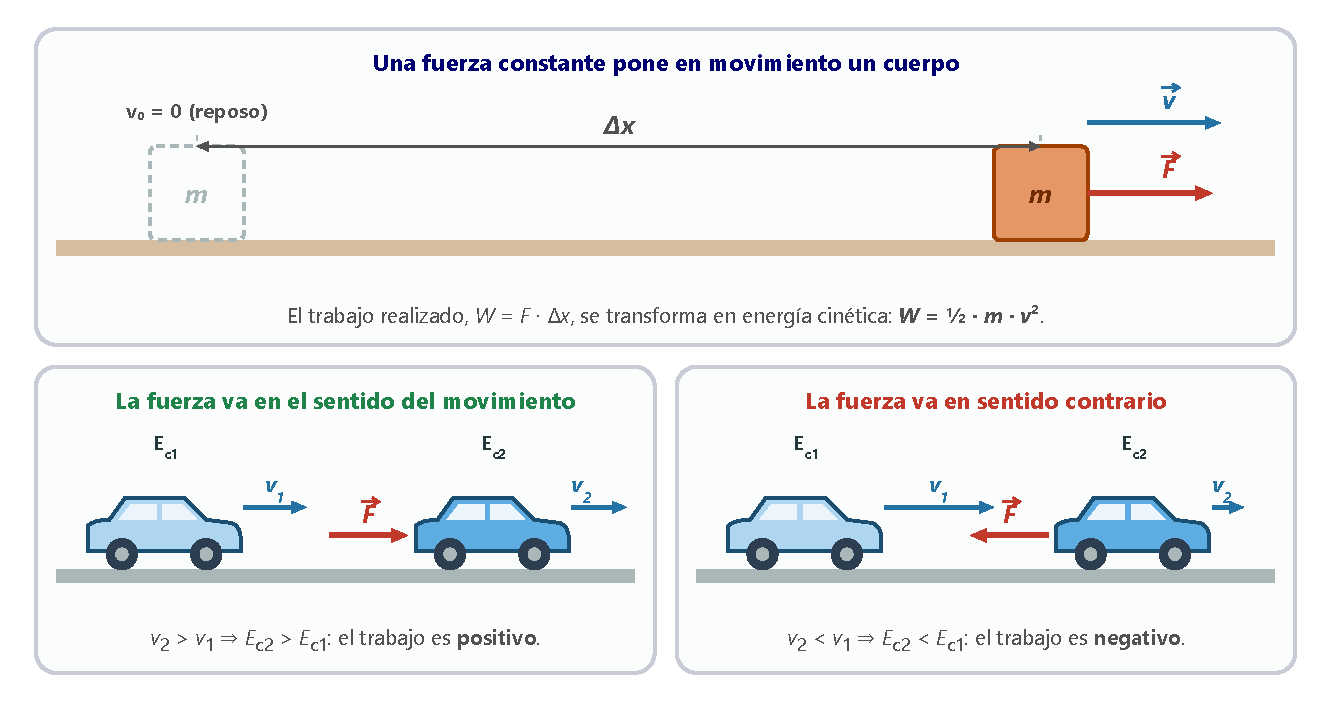
\includegraphics[width=\textwidth]{images/UD11/energia_cinetica}
    \caption{El trabajo realizado sobre un cuerpo se transforma en energía cinética.}
    \label{fig:energia_cinetica}
\end{figure}

\paragraph{¿Qué relación hay entre el trabajo y la variación de energía cinética?} Si un cuerpo ya se mueve y le aplicamos una fuerza, su velocidad puede aumentar o disminuir.

\begin{definition}[Teorema de la energía cinética]
    El trabajo realizado por la resultante de todas las fuerzas que actúan sobre un cuerpo es igual a la variación de su energía cinética:
    \[ W = E_{c2} - E_{c1} = \Delta E_c \]
\end{definition}

Si la fuerza resultante tiene el sentido del movimiento, la velocidad aumenta, \(E_{c2} > E_{c1}\), y el trabajo es \textbf{positivo}. Si tiene sentido contrario (por ejemplo, al frenar), la velocidad disminuye, \(E_{c2} < E_{c1}\), y el trabajo es \textbf{negativo}.

\begin{example}
    Una vagoneta de \qty{100}{\kg} se mueve en línea recta a \qty{2}{\m\per\s}. Le aplicamos una fuerza y, tras recorrer \qty{5}{\m}, su velocidad es de \qty{4}{\m\per\s}. Si no hay rozamiento, calcula el trabajo realizado y el valor de la fuerza.

    \(E_{c1} = \frac{1}{2} \cdot 100 \cdot 2^2 = \qty{200}{\joule}\); \quad \(E_{c2} = \frac{1}{2} \cdot 100 \cdot 4^2 = \qty{800}{\joule}\).
    \[ W = \Delta E_c = 800 - 200 = \textcolor{red}{\qty{600}{\joule}} \qquad F = \frac{W}{\Delta x} = \frac{600}{5} = \textcolor{red}{\qty{120}{\newton}} \]
\end{example}

\begin{exercise}
    Escribe la ecuación de dimensiones de la energía cinética y comprueba que coincide con la del trabajo. ¿Es una ecuación homogénea?
    \begin{solu}
        \([E_c] = [m] \cdot [v]^2 = \mathrm{M} \cdot (\mathrm{L \cdot T^{-1}})^2 = \textcolor{red}{\mathrm{M \cdot L^2 \cdot T^{-2}}}\), igual que la del trabajo: la ecuación \(W = \frac{1}{2} m v^2\) \textcolor{red}{es homogénea}.
    \end{solu}
\end{exercise}

\begin{exercise}
    Un cuerpo de \qty{50}{\kg} se mueve a \qty{2}{\m\per\s}. ¿Qué energía cinética tiene? ¿Cuánto aumentaría si se duplicara su masa? ¿Y si se duplicara su velocidad?
    \begin{solu}
        \(E_c = \frac{1}{2} \cdot 50 \cdot 2^2 = \textcolor{red}{\qty{100}{\joule}}\). Si se duplica la masa, la energía cinética \textcolor{red}{se duplica} (\qty{200}{\joule}); si se duplica la velocidad, \textcolor{red}{se cuadruplica} (\qty{400}{\joule}).
    \end{solu}
\end{exercise}

\begin{exercise}
    ¿Puede ser negativa la energía cinética de un cuerpo? ¿Y su variación?
    \begin{solu}
        La energía cinética \textcolor{red}{no puede ser negativa}: la masa es positiva y la velocidad está elevada al cuadrado. Su variación \textcolor{red}{sí puede ser negativa}, cuando el cuerpo pierde velocidad (por ejemplo, al frenar).
    \end{solu}
\end{exercise}

\begin{exercise}
    Calcula la energía cinética de un vehículo de \qty{500}{\kg} que circula a \qty{90}{\km\per\hour}.
    \begin{solu}
        \(v = \qty{90}{\km\per\hour} = \qty{25}{\m\per\s}\); \(E_c = \frac{1}{2} \cdot 500 \cdot 25^2 = \textcolor{red}{\qty{1.56e5}{\joule}}\).
    \end{solu}
\end{exercise}

\begin{exercise}
    Un vehículo de \qty{600}{\kg} que circula por una carretera recta y horizontal pasa de \qty{10}{\m\per\s} a \qty{20}{\m\per\s} en \qty{10}{\m}. Calcula la fuerza resultante que ha actuado sobre él.
    \begin{solu}
        \(E_{c1} = \frac{1}{2} \cdot 600 \cdot 10^2 = \qty{30000}{\joule}\); \(E_{c2} = \frac{1}{2} \cdot 600 \cdot 20^2 = \qty{120000}{\joule}\).
        \(W = \Delta E_c = \qty{90000}{\joule}\); \(F = \dfrac{W}{\Delta x} = \dfrac{90000}{10} = \textcolor{red}{\qty{9000}{\newton}}\).
    \end{solu}
\end{exercise}

\subsection{¿Puede un cuerpo en reposo tener energía mecánica? La energía potencial}

Un saltador de trampolín en lo alto de la plataforma está quieto, pero tiene energía: cuando salte, su peso realizará un trabajo y ganará velocidad.

\begin{definition}[Energía potencial]
    La \textbf{energía potencial}, \(E_p\), es la energía que tiene un cuerpo debido a la posición que ocupa, distinta de su posición de equilibrio.
\end{definition}

\paragraph{La energía potencial gravitatoria.} Cuando una roca de masa \(m\) cae desde una altura \(h\) (figura~\ref{fig:energia_potencial}), su peso y el desplazamiento tienen la misma dirección y sentido, así que el peso realiza un trabajo positivo:
\[ W = m \cdot g \cdot h \]
Este trabajo es igual a la \textbf{disminución} de la energía potencial: \(W = -\Delta E_p = E_{p1} - E_{p2}\). Solo podemos calcular diferencias de energía potencial, así que tomamos por convenio como nivel cero el suelo (\(h = 0\)). Entonces, \(E_{p2} = 0\) y \(W = E_{p1} = m \cdot g \cdot h\).

\begin{definition}[Energía potencial gravitatoria]
    La energía potencial gravitatoria de un cuerpo de masa \(m\) situado a una altura \(h\) sobre el nivel de referencia es:
    \[ E_p = m \cdot g \cdot h \]
\end{definition}

Para \textbf{subir} la roca desde el suelo hasta la altura \(h\), el peso y el desplazamiento tienen sentidos opuestos: el peso realiza un trabajo negativo, \(W = -m \cdot g \cdot h\), y nosotros tenemos que realizar un trabajo \(m \cdot g \cdot h\), que queda almacenado como energía potencial. Este trabajo \textbf{no depende del camino seguido}, sino solo de la diferencia de altura.

\begin{figure}[H]
    \centering
    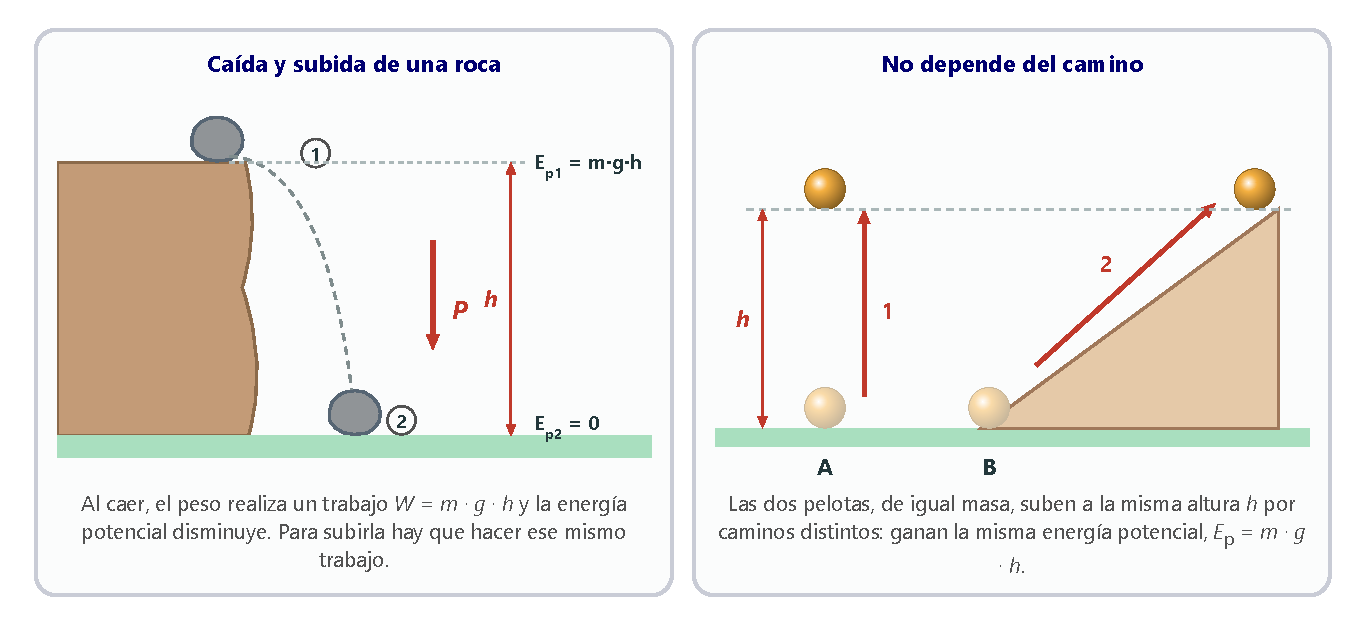
\includegraphics[width=\textwidth]{images/UD11/energia_potencial}
    \caption{La energía potencial gravitatoria depende solo de la altura.}
    \label{fig:energia_potencial}
\end{figure}

\paragraph{La energía potencial elástica.} Para estirar o comprimir un muelle una distancia \(x\) hay que aplicar una fuerza que cumple la \textbf{ley de Hooke}: \(F = k \cdot x\), donde \(k\) es la constante elástica del muelle (figura~\ref{fig:muelle}). El trabajo realizado no se convierte en energía cinética (el muelle se estira despacio) ni en energía potencial gravitatoria (el movimiento es horizontal): queda almacenado en el muelle deformado.

\begin{figure}[H]
    \centering
    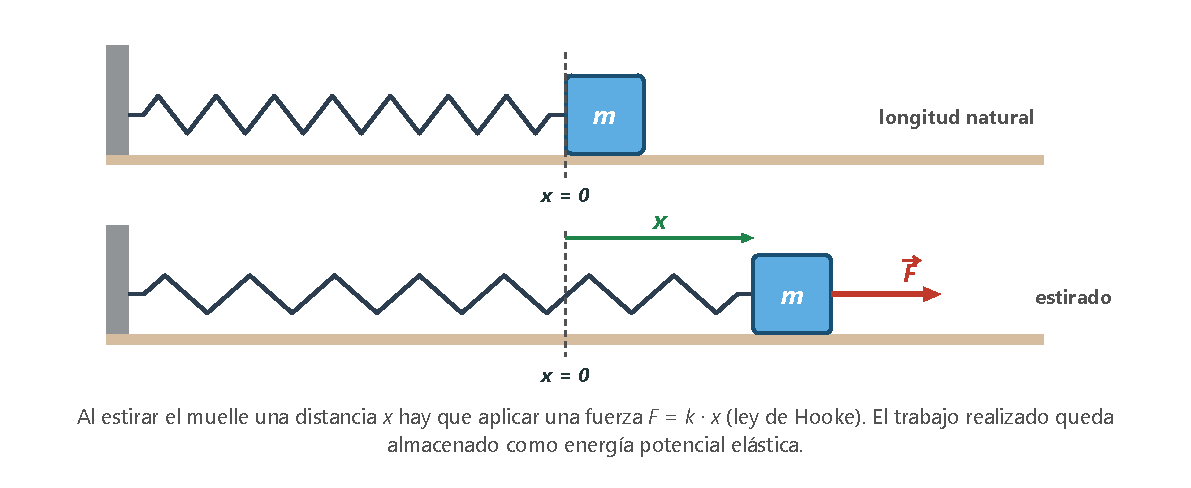
\includegraphics[width=0.85\textwidth]{images/UD11/muelle}
    \caption{Un muelle estirado almacena energía potencial elástica.}
    \label{fig:muelle}
\end{figure}

Como la fuerza no es constante, el trabajo se calcula como el área bajo la gráfica \(F\)--\(x\), que es un triángulo de base \(x\) y altura \(k \cdot x\):
\[ W = \frac{1}{2} \cdot x \cdot (k \cdot x) = \frac{1}{2} \cdot k \cdot x^2 \]

\begin{center}
    \begin{tikzpicture}
        \begin{axis}[grafica, width=7cm, height=5cm, xlabel={alargamiento, \(x\)}, ylabel={fuerza, \(F\)}, xmin=0, xmax=5.5, ymin=0, ymax=5.5, xticklabels={}, yticklabels={}]
            \addplot[mark=none, fill=red!20, draw=red!75!black, line width=1.4pt] coordinates {(0,0) (4,4) (4,0)};
            \node at (axis cs:2.4,0.6) {\small área \(= \frac{1}{2} \cdot b \cdot h\)};
            \node[anchor=west] at (axis cs:4.05,4) {\small \(F = k \cdot x\)};
        \end{axis}
    \end{tikzpicture}
\end{center}

\begin{definition}[Energía potencial elástica]
    La \textbf{energía potencial elástica} es la que tiene un cuerpo elástico (un muelle, una goma\ldots) cuando está estirado o comprimido. Si cumple la ley de Hooke:
    \[ E_p = \frac{1}{2} \cdot k \cdot x^2 \]
    Es proporcional al \textbf{cuadrado} de la deformación.
\end{definition}

\begin{example}
    Calcula la energía potencial elástica de un muelle de constante \qty{100}{\newton\per\m} comprimido \qty{4}{\cm} desde su longitud natural.
    \[ E_p = \frac{1}{2} \cdot k \cdot x^2 = \frac{1}{2} \cdot 100 \cdot (\num{0.04})^2 = \textcolor{red}{\qty{0.08}{\joule}} \]
\end{example}

\begin{exercise}
    Calcula la energía potencial de un saltador de trampolín de \qty{75}{\kg} situado a \qty{10}{\m} sobre el agua. ¿Qué trabajo realiza su peso cuando cae a la piscina?
    \begin{solu}
        \(E_p = m \cdot g \cdot h = 75 \cdot \num{9.8} \cdot 10 = \textcolor{red}{\qty{7350}{\joule}}\). El peso realiza ese mismo trabajo al caer: \(W = \textcolor{red}{\qty{7350}{\joule}}\).
    \end{solu}
\end{exercise}

\begin{exercise}
    Un cuerpo de \qty{10}{\kg} está a \qty{4}{\m} de altura. ¿Qué trabajo realiza su peso cuando cae hasta el suelo?
    \begin{solu}
        \(W = -\Delta E_p = m \cdot g \cdot h = 10 \cdot \num{9.8} \cdot 4 = \textcolor{red}{\qty{392}{\joule}}\).
    \end{solu}
\end{exercise}

\begin{exercise}
    Al estirar un muelle, la fuerza aumenta de forma proporcional al alargamiento, como en la gráfica. Calcula el trabajo realizado. ¿Qué energía potencial elástica ha adquirido el muelle?
    \begin{center}
        \begin{tikzpicture}
            \begin{axis}[grafica, width=6.5cm, height=4.2cm, xlabel={\(x\) (cm)}, ylabel={\(F\) (N)}, xmin=0, xmax=6, ymin=0, ymax=5, xtick={0,2,4,6}, ytick={0,2,4}]
                \addplot[mark=none, fill=red!20, draw=red!75!black, line width=1.4pt] coordinates {(0,0) (4,4) (4,0)};
            \end{axis}
        \end{tikzpicture}
    \end{center}
    \begin{solu}
        El trabajo es el área del triángulo: \(W = \frac{1}{2} \cdot \num{0.04} \cdot 4 = \textcolor{red}{\qty{0.08}{\joule}}\). Esa es la energía potencial elástica que ha adquirido el muelle: \(E_p = \textcolor{red}{\qty{0.08}{\joule}}\).
    \end{solu}
\end{exercise}

\begin{exercise}
    Un muelle de constante \qty{50}{\newton\per\m} se estira hasta que su energía potencial elástica es \qty{6.25e-2}{\joule}. ¿Cuánto se ha estirado? ¿Cuánto varía su energía potencial cuando vuelve a su longitud natural?
    \begin{solu}
        \(\num{6.25e-2} = \frac{1}{2} \cdot 50 \cdot x^2 \Rightarrow x^2 = \num{2.5e-3} \Rightarrow x = \textcolor{red}{\qty{0.05}{\m}} = \qty{5}{\cm}\).
        Al volver a su longitud natural, \(\Delta E_p = 0 - \num{6.25e-2} = \textcolor{red}{\qty{-6.25e-2}{\joule}}\).
    \end{solu}
\end{exercise}

\begin{exercise}
    Comprueba que la ecuación \(E_p = m \cdot g \cdot h\) es homogénea.
    \begin{solu}
        \([m \cdot g \cdot h] = \mathrm{M} \cdot \mathrm{L \cdot T^{-2}} \cdot \mathrm{L} = \mathrm{M \cdot L^2 \cdot T^{-2}}\), que son las dimensiones de una energía: \textcolor{red}{es homogénea}.
    \end{solu}
\end{exercise}

\subsection*{Actividades de consolidación: energía mecánica}

\begin{exercise}
    Indica si son verdaderas o falsas estas afirmaciones:
    \begin{enumerate}[label=\alph*)]
        \item La energía cinética depende de la masa del cuerpo y de su velocidad.
        \item Un cuerpo en reposo puede tener energía mecánica.
        \item Si B tiene la misma masa que A y el doble de velocidad, tiene el doble de energía cinética.
        \item La energía cinética de un cuerpo puede ser negativa.
        \item La variación de energía cinética puede ser negativa.
        \item La energía potencial elástica es proporcional al cuadrado de la deformación.
        \item El trabajo realizado por el peso es igual a la disminución de la energía potencial gravitatoria.
    \end{enumerate}
    \begin{solu}
        a) \textcolor{red}{V}. b) \textcolor{red}{V} (energía potencial). c) \textcolor{red}{F}: tiene cuatro veces más. d) \textcolor{red}{F}. e) \textcolor{red}{V}. f) \textcolor{red}{V}. g) \textcolor{red}{V}.
    \end{solu}
\end{exercise}

\begin{exercise}
    ¿Cuánto varía la energía cinética de un atleta de \qty{60}{\kg} cuando su velocidad pasa de \qty{1.5}{\m\per\s} a \qty{2.75}{\m\per\s}?
    \begin{solu}
        \(E_{c1} = \frac{1}{2} \cdot 60 \cdot \num{1.5}^2 = \qty{67.5}{\joule}\); \(E_{c2} = \frac{1}{2} \cdot 60 \cdot \num{2.75}^2 = \qty{226.9}{\joule}\); \(\Delta E_c = \textcolor{red}{\qty{159.4}{\joule}}\).
    \end{solu}
\end{exercise}

\begin{exercise}
    Un bloque de piedra de \qty{100}{\kg}, en reposo sobre un plano liso y horizontal, es empujado con una fuerza constante de \qty{25}{\newton} a lo largo de \qty{25}{\m}. Calcula la energía cinética y la velocidad que adquiere.
    \begin{solu}
        \(E_c = W = 25 \cdot 25 = \textcolor{red}{\qty{625}{\joule}}\); \(v = \sqrt{\dfrac{2 E_c}{m}} = \sqrt{\dfrac{2 \cdot 625}{100}} = \textcolor{red}{\qty{3.54}{\m\per\s}}\).
    \end{solu}
\end{exercise}

\begin{exercise}
    Un vehículo de \qty{500}{\kg} circula a \qty{100}{\km\per\hour} y frena hasta detenerse. ¿Cuánto varía su energía cinética? ¿Qué trabajo realiza la fuerza de frenado?
    \begin{solu}
        \(v = \qty{27.8}{\m\per\s}\); \(E_c = \frac{1}{2} \cdot 500 \cdot \num{27.8}^2 = \qty{1.93e5}{\joule}\). \(\Delta E_c = 0 - \num{1.93e5} = \textcolor{red}{\qty{-1.93e5}{\joule}}\), que es el trabajo de la fuerza de frenado: \(W = \textcolor{red}{\qty{-1.93e5}{\joule}}\).
    \end{solu}
\end{exercise}

\begin{exercise}
    Si el trabajo realizado por la fuerza resultante sobre un cuerpo es nulo, su energía cinética es: a) nula; b) constante.
    \begin{solu}
        \textcolor{red}{b) constante}, porque \(W = \Delta E_c = 0\).
    \end{solu}
\end{exercise}

\begin{exercise}
    Un halcón en vuelo tiene más energía cinética que un águila, aunque el águila tiene más masa. ¿Cómo es posible?
    \begin{solu}
        Porque la energía cinética depende del \textcolor{red}{cuadrado de la velocidad}: el halcón vuela mucho más rápido, y eso compensa su menor masa.
    \end{solu}
\end{exercise}

\begin{exercise}
    Un cuerpo de \qty{1}{\kg} se mueve a \qty{2}{\m\per\s}. ¿Qué trabajo hay que realizar sobre él para pararlo?
    \begin{solu}
        \(W = \Delta E_c = 0 - \frac{1}{2} \cdot 1 \cdot 2^2 = \textcolor{red}{\qty{-2}{\joule}}\): hay que quitarle \qty{2}{\joule} con una fuerza de sentido contrario al movimiento.
    \end{solu}
\end{exercise}

\begin{exercise}
    Una maleta de \qty{8}{\kg}, inicialmente en reposo, es empujada con una fuerza de \qty{16}{\newton} por un suelo horizontal sin rozamiento y se desplaza \qty{4}{\m}. Calcula: a) el trabajo de la fuerza; b) la variación de energía cinética; c) la velocidad final.
    \begin{solu}
        a) \(W = 16 \cdot 4 = \textcolor{red}{\qty{64}{\joule}}\). b) \(\Delta E_c = W = \textcolor{red}{\qty{64}{\joule}}\). c) \(v = \sqrt{\dfrac{2 \cdot 64}{8}} = \textcolor{red}{\qty{4}{\m\per\s}}\).
    \end{solu}
\end{exercise}

\begin{exercise}
    Un coche recorre \qty{2}{\km} por una carretera horizontal y su energía cinética aumenta \qty{20000}{\joule}. ¿Qué trabajo neto se ha realizado sobre él?
    \begin{solu}
        \(W = \Delta E_c = \textcolor{red}{\qty{20000}{\joule}}\) (es el trabajo de la fuerza resultante: el del motor menos el que se pierde por rozamiento).
    \end{solu}
\end{exercise}

\begin{exercise}
    ¿Cómo varía la energía potencial gravitatoria en un desplazamiento horizontal?
    \begin{solu}
        \textcolor{red}{No varía}, porque la altura es la misma.
    \end{solu}
\end{exercise}

\begin{exercise}
    En una escalera de peldaños de \qty{15}{\cm}, las posiciones 1, 2 y 3 están a \qty{0.15}{\m}, \qty{0.45}{\m} y \qty{0.75}{\m} del suelo. Un cuerpo A, de \qty{2}{\kg}, está en la posición 3, y un cuerpo B, de \qty{1}{\kg}, en la posición 1. a) ¿Qué energía potencial tiene cada uno? b) ¿Qué trabajo hay que hacer para subir B de la posición 1 a la 2? c) ¿Cuánto varía la energía potencial de A al bajar de la posición 3 a la 2?
    \begin{solu}
        a) \(E_{pA} = 2 \cdot \num{9.8} \cdot \num{0.75} = \textcolor{red}{\qty{14.7}{\joule}}\); \(E_{pB} = 1 \cdot \num{9.8} \cdot \num{0.15} = \textcolor{red}{\qty{1.47}{\joule}}\).
        b) \(W = 1 \cdot \num{9.8} \cdot (\num{0.45} - \num{0.15}) = \textcolor{red}{\qty{2.94}{\joule}}\).
        c) \(\Delta E_p = 2 \cdot \num{9.8} \cdot (\num{0.45} - \num{0.75}) = \textcolor{red}{\qty{-5.88}{\joule}}\).
    \end{solu}
\end{exercise}

\begin{exercise}
    Una grúa eleva una viga de \qty{100}{\kg} desde el suelo hasta \qty{20}{\m} de altura. a) ¿Qué trabajo realiza? b) ¿Qué energía potencial tiene la viga en el suelo y a \qty{20}{\m}? c) ¿A qué equivale su variación de energía potencial?
    \begin{solu}
        a) \(W = 100 \cdot \num{9.8} \cdot 20 = \textcolor{red}{\qty{19600}{\joule}}\). b) En el suelo, \textcolor{red}{\qty{0}{\joule}}; a \qty{20}{\m}, \textcolor{red}{\qty{19600}{\joule}}. c) \textcolor{red}{Al trabajo realizado} por la grúa para subirla.
    \end{solu}
\end{exercise}

\begin{exercise}
    Queremos subir un cuerpo de \qty{10}{\kg} desde el suelo. a) ¿Qué energía potencial tiene en el suelo? b) ¿Y a \qty{4}{\m} de altura? c) ¿Qué trabajo hay que hacer para subirlo? d) ¿Cuándo es negativa la variación de energía potencial?
    \begin{solu}
        a) \textcolor{red}{\qty{0}{\joule}}. b) \(E_p = 10 \cdot \num{9.8} \cdot 4 = \textcolor{red}{\qty{392}{\joule}}\). c) \(W = \Delta E_p = \textcolor{red}{\qty{392}{\joule}}\). d) Cuando el cuerpo \textcolor{red}{baja}: la energía potencial final es menor que la inicial.
    \end{solu}
\end{exercise}

\begin{exercise}
    Calcula la energía potencial elástica de un muelle de constante \qty{2000}{\newton\per\m} estirado \qty{2}{\cm}.
    \begin{solu}
        \(E_p = \frac{1}{2} \cdot 2000 \cdot (\num{0.02})^2 = \textcolor{red}{\qty{0.4}{\joule}}\).
    \end{solu}
\end{exercise}

\begin{exercise}
    Dos pelotas iguales, A y B, suben a la misma altura \(h\): A, verticalmente; B, rodando por una rampa (figura~\ref{fig:energia_potencial}). a) ¿Qué energía potencial adquiere cada una? b) ¿Qué trabajo se ha hecho para subirlas? c) ¿Qué conclusión se obtiene?
    \begin{solu}
        a) Las dos, \textcolor{red}{la misma}: \(E_p = m \cdot g \cdot h\). b) El mismo, \(W = m \cdot g \cdot h\) (sin rozamiento). c) El trabajo para subir un cuerpo \textcolor{red}{no depende del camino}, solo de la altura.
    \end{solu}
\end{exercise}

\begin{exercise}
    Calcula la energía potencial elástica de un muelle de constante \qty{100}{\newton\per\m} comprimido \qty{5}{\cm}.
    \begin{solu}
        \(E_p = \frac{1}{2} \cdot 100 \cdot (\num{0.05})^2 = \textcolor{red}{\qty{0.125}{\joule}}\).
    \end{solu}
\end{exercise}

\begin{exercise}
    La fuerza de la gráfica no es constante. Calcula el trabajo que realiza entre \(x = 0\) y \(x = \qty{8}{\m}\).
    \begin{center}
        \begin{tikzpicture}
            \begin{axis}[grafica, width=8cm, height=4.4cm, xlabel={\(x\) (m)}, ylabel={\(F\) (N)}, xmin=0, xmax=8.6, ymin=0, ymax=75, xtick={0,2,...,8}, ytick={0,20,40,60}]
                \addplot[mark=none, fill=red!20, draw=red!75!black, line width=1.4pt] coordinates {(0,0) (2,60) (4,60) (8,0)};
            \end{axis}
        \end{tikzpicture}
    \end{center}
    \begin{solu}
        El trabajo es el área bajo la gráfica: un triángulo, un rectángulo y otro triángulo.
        \(W = \frac{1}{2} \cdot 2 \cdot 60 + 2 \cdot 60 + \frac{1}{2} \cdot 4 \cdot 60 = 60 + 120 + 120 = \textcolor{red}{\qty{300}{\joule}}\).
    \end{solu}
\end{exercise}

\begin{exercise}
    Una joven de \qty{65}{\kg} sube a una torre de \qty{93}{\m}. a) ¿Qué trabajo realiza? b) ¿Qué energía potencial tiene arriba?
    \begin{solu}
        a) \(W = 65 \cdot \num{9.8} \cdot 93 = \textcolor{red}{\qty{59241}{\joule}}\). b) La misma: \(E_p = \textcolor{red}{\qty{59241}{\joule}}\).
    \end{solu}
\end{exercise}

\begin{exercise}
    Un cuerpo de \qty{8}{\kg} cae desde \qty{20}{\m}. ¿Cuánto varía su energía potencial? ¿Qué trabajo realiza el peso?
    \begin{solu}
        \(\Delta E_p = 0 - 8 \cdot \num{9.8} \cdot 20 = \textcolor{red}{\qty{-1568}{\joule}}\); el peso realiza un trabajo \(W = -\Delta E_p = \textcolor{red}{\qty{1568}{\joule}}\).
    \end{solu}
\end{exercise}

%========================================================================================
\section[Conservación de la energía mecánica]{El principio de conservación de la energía mecánica}
%========================================================================================

\begin{definition}[Energía mecánica]
    La \textbf{energía mecánica}, \(E_m\), es la suma de la energía cinética y la energía potencial de un cuerpo:
    \[ E_m = E_c + E_p \]
\end{definition}

\subsection{¿Cómo se transforma la energía potencial en cinética y viceversa?}

Una niña de \qty{25}{\kg} está sentada, en reposo, en lo alto de un tobogán de \qty{2}{\m} (figura~\ref{fig:conservacion}). No tiene energía cinética, y su energía potencial es \(E_p = 25 \cdot \num{9.8} \cdot 2 = \qty{490}{\joule}\). Mientras baja, su energía potencial disminuye y su energía cinética aumenta. A mitad de altura (\(h = \qty{1}{\m}\)), \(E_p = \qty{245}{\joule}\) y \(E_c = \qty{245}{\joule}\); al llegar abajo, toda la energía potencial se ha transformado en cinética: \(E_c = \qty{490}{\joule}\). En todo momento, la suma de las dos es \qty{490}{\joule}.

\begin{definition}[Principio de conservación de la energía mecánica]
    Si no hay rozamiento, la suma de la energía cinética y la energía potencial de un cuerpo permanece constante en todos los puntos de su trayectoria:
    \[ E_m = E_c + E_p = \text{constante} \]
\end{definition}

\begin{figure}[H]
    \centering
    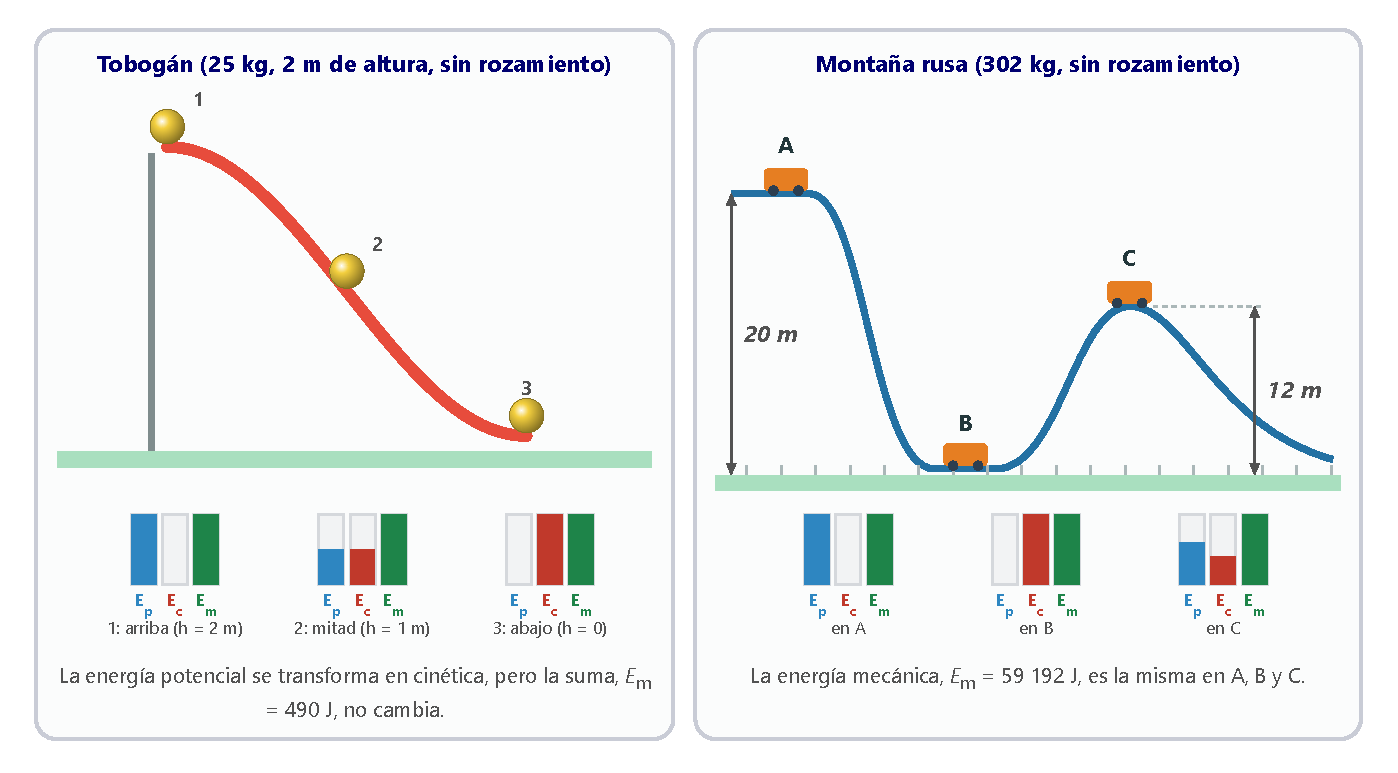
\includegraphics[width=\textwidth]{images/UD11/conservacion}
    \caption{Conservación de la energía mecánica en un tobogán y en una montaña rusa.}
    \label{fig:conservacion}
\end{figure}

Gracias a este principio podemos calcular velocidades sin conocer las fuerzas. Por ejemplo, la velocidad de la niña al final del tobogán:
\[ E_c = \frac{1}{2} \cdot m \cdot v^2 \quad\Rightarrow\quad v = \sqrt{\frac{2 E_c}{m}} = \sqrt{\frac{2 \cdot 490}{25}} = \qty{6.26}{\m\per\s} \]
Si toda la energía potencial se transforma en cinética, \(m \cdot g \cdot h = \frac{1}{2} \cdot m \cdot v^2\), y la velocidad final es \(v = \sqrt{2 \cdot g \cdot h}\): no depende de la masa.

\subsection{Aplicaciones del principio de conservación de la energía mecánica}

\begin{example}
    \textbf{Viaje en caída libre.} En una atracción, el vehículo y su pasajero (\qty{248}{\kg} en total) suben hasta \qty{50}{\m} y se dejan caer. Despreciando el rozamiento, calcula la energía mecánica y la velocidad con que llegan abajo, antes de frenar.

    Arriba, en reposo: \(E_m = E_p = 248 \cdot \num{9.8} \cdot 50 = \textcolor{red}{\qty{121520}{\joule}}\). Abajo, toda es cinética:
    \[ v = \sqrt{\frac{2 E_c}{m}} = \sqrt{\frac{2 \cdot 121520}{248}} = \textcolor{red}{\qty{31.3}{\m\per\s}} \quad (\text{más de } \qty{110}{\km\per\hour}) \]
\end{example}

\begin{example}
    \textbf{Viaje en montaña rusa.} Un vagón con su pasajero (\qty{302}{\kg}) parte del reposo en el punto A, a \qty{20}{\m} de altura, baja hasta el punto B, al nivel del suelo, y sube al punto C, a \qty{12}{\m} (figura~\ref{fig:conservacion}). Sin rozamiento, calcula la energía mecánica y las energías cinética y potencial en B y en C.

    En A: \(E_m = E_p = 302 \cdot \num{9.8} \cdot 20 = \textcolor{red}{\qty{59192}{\joule}}\), y se conserva en todo el recorrido.

    En B (\(h = 0\)): \(E_p = 0\) y \(E_c = \textcolor{red}{\qty{59192}{\joule}}\), el valor máximo.

    En C: \(E_p = 302 \cdot \num{9.8} \cdot 12 = \textcolor{red}{\qty{35515}{\joule}}\); \(E_c = 59192 - 35515 = \textcolor{red}{\qty{23677}{\joule}}\).
\end{example}

\begin{exercise}
    Un cuerpo de \qty{1}{\kg} se deja caer desde una torre. ¿Qué tipo de energía tiene en el momento en que está a \qty{10}{\m} del suelo: potencial, cinética o ambas?
    \begin{solu}
        \textcolor{red}{Ambas}: potencial, porque aún está a cierta altura, y cinética, porque ya se mueve. Al soltarlo solo tenía energía potencial, y al llegar al suelo solo tendrá cinética.
    \end{solu}
\end{exercise}

\begin{exercise}
    Un bloque de \qty{2}{\kg} se desliza sin rozamiento a \qty{2}{\m\per\s} y choca contra un muelle de constante \qty{100}{\newton\per\m}. ¿Cuánto se comprime el muelle?
    \begin{solu}
        Toda la energía cinética se transforma en potencial elástica:
        \(\frac{1}{2} \cdot 2 \cdot 2^2 = \frac{1}{2} \cdot 100 \cdot x^2 \Rightarrow 4 = 50 \, x^2 \Rightarrow x = \textcolor{red}{\qty{0.28}{\m}} = \qty{28}{\cm}\).
    \end{solu}
\end{exercise}

\begin{exercise}
    En la atracción de caída libre del ejemplo anterior, ¿qué energía potencial y cinética tiene el vehículo cuando está a \qty{10}{\m} del suelo? ¿Y qué energía mecánica?
    \begin{solu}
        \(E_p = 248 \cdot \num{9.8} \cdot 10 = \textcolor{red}{\qty{24304}{\joule}}\); \(E_c = 121520 - 24304 = \textcolor{red}{\qty{97216}{\joule}}\). La energía mecánica es la misma que en todo el recorrido: \(E_m = \textcolor{red}{\qty{121520}{\joule}}\).
    \end{solu}
\end{exercise}

\subsection*{Actividades de consolidación: conservación de la energía mecánica}

\begin{exercise}
    ¿En qué se transforma la energía potencial elástica de un juguete de cuerda?
    \begin{solu}
        En \textcolor{red}{energía cinética} del juguete (y, por los rozamientos, en energía térmica).
    \end{solu}
\end{exercise}

\begin{exercise}
    Un cuerpo en reposo a cierta altura se deja caer libremente. a) ¿Qué energía tiene al principio? b) ¿Qué ocurre con su energía cinética durante la caída? c) ¿Qué energía tiene al llegar al suelo?
    \begin{solu}
        a) Solo \textcolor{red}{potencial gravitatoria}. b) \textcolor{red}{Aumenta}, a medida que disminuye la potencial. c) Solo \textcolor{red}{cinética}.
    \end{solu}
\end{exercise}

\begin{exercise}
    Un péndulo tiene una masa de \qty{2}{\kg} y un hilo de \qty{0.5}{\m}. a) ¿Qué trabajo hay que hacer para llevarlo desde su posición de equilibrio hasta la horizontal? b) Si se suelta desde la horizontal, ¿con qué velocidad pasa por la posición de equilibrio?
    \begin{solu}
        a) La bola sube una altura igual a la longitud del hilo: \(W = m \cdot g \cdot h = 2 \cdot \num{9.8} \cdot \num{0.5} = \textcolor{red}{\qty{9.8}{\joule}}\).
        b) \(\frac{1}{2} \cdot m \cdot v^2 = \qty{9.8}{\joule} \Rightarrow v = \sqrt{\dfrac{2 \cdot \num{9.8}}{2}} = \textcolor{red}{\qty{3.13}{\m\per\s}}\).
    \end{solu}
\end{exercise}

\begin{exercise}
    Un cuerpo de \qty{10}{\kg} se lanza verticalmente hacia arriba a \qty{25}{\m\per\s}. Aplicando la conservación de la energía, calcula la altura máxima que alcanza.
    \begin{solu}
        \(\frac{1}{2} \cdot m \cdot v^2 = m \cdot g \cdot h \Rightarrow h = \dfrac{v^2}{2g} = \dfrac{25^2}{2 \cdot \num{9.8}} = \textcolor{red}{\qty{31.9}{\m}}\).
    \end{solu}
\end{exercise}

\begin{exercise}
    Un cuerpo de \qty{100}{\gram}, sujeto a un muelle de constante \qty{200}{\newton\per\m}, está apoyado en un plano horizontal sin rozamiento. Lo separamos \qty{10}{\cm} de su posición de equilibrio y lo soltamos. a) ¿Qué energía potencial tiene al principio? b) ¿Cuál es su energía mecánica? c) ¿Con qué velocidad pasa por la posición de equilibrio?
    \begin{solu}
        a) \(E_p = \frac{1}{2} \cdot 200 \cdot \num{0.1}^2 = \textcolor{red}{\qty{1}{\joule}}\). b) \(E_m = \textcolor{red}{\qty{1}{\joule}}\) durante todo el movimiento.
        c) \(\frac{1}{2} \cdot \num{0.1} \cdot v^2 = 1 \Rightarrow v = \sqrt{20} = \textcolor{red}{\qty{4.47}{\m\per\s}}\).
    \end{solu}
\end{exercise}

\begin{exercise}
    Por una presa con un desnivel de \qty{65}{\m} caen \qty{250}{\cubic\m} de agua por minuto. ¿Cuánta energía puede proporcionar el agua cada minuto? ¿Qué potencia supone?
    \begin{solu}
        \(m = \qty{250000}{\kg}\); \(E_p = 250000 \cdot \num{9.8} \cdot 65 = \textcolor{red}{\qty{1.6e8}{\joule}}\) por minuto.
        \(P = \dfrac{\num{1.6e8}}{60} = \textcolor{red}{\qty{2.7e6}{\watt}} = \qty{2.7}{\mega\watt}\).
    \end{solu}
\end{exercise}

\begin{exercise}
    Un cuerpo de \qty{10}{\kg} cae desde \qty{20}{\m}. a) ¿Qué energía potencial tiene a \qty{10}{\m} de altura? b) ¿Qué velocidad tiene en ese instante? c) ¿Qué trabajo realiza el peso hasta que llega al suelo? d) ¿Con qué velocidad llega al suelo?
    \begin{solu}
        a) \(E_p = 10 \cdot \num{9.8} \cdot 10 = \textcolor{red}{\qty{980}{\joule}}\).
        b) \(E_m = 10 \cdot \num{9.8} \cdot 20 = \qty{1960}{\joule}\), así que \(E_c = 1960 - 980 = \qty{980}{\joule}\) y \(v = \sqrt{\dfrac{2 \cdot 980}{10}} = \textcolor{red}{\qty{14}{\m\per\s}}\).
        c) \(W = m \cdot g \cdot h = \textcolor{red}{\qty{1960}{\joule}}\). d) \(v = \sqrt{\dfrac{2 \cdot 1960}{10}} = \textcolor{red}{\qty{19.8}{\m\per\s}}\).
    \end{solu}
\end{exercise}

\begin{exercise}
    Se deja caer una bola de \qty{4}{\kg} desde el punto A de una rampa, a \qty{2}{\m} de altura. La rampa baja hasta un tramo horizontal (puntos B y C, a nivel del suelo) y vuelve a subir. a) ¿Qué energía tiene en B y en C? b) Si no hay rozamiento, ¿qué altura alcanza en la rampa de subida?
    \begin{solu}
        a) En B y en C solo tiene \textcolor{red}{energía cinética}, igual a la potencial que tenía en A: \(E_c = 4 \cdot \num{9.8} \cdot 2 = \textcolor{red}{\qty{78.4}{\joule}}\).
        b) Sube hasta la \textcolor{red}{misma altura}, \qty{2}{\m}, porque la energía mecánica se conserva.
    \end{solu}
\end{exercise}

%========================================================================================
\section[Conservación de la energía total]{El principio general de conservación de la energía total}
%========================================================================================

Si dejamos caer una canica desde el borde de un cuenco, su energía potencial se transforma en cinética al bajar, y la cinética otra vez en potencial al subir por el otro lado. ¿Se repite indefinidamente? La experiencia dice que no: en cada oscilación la canica sube un poco menos, hasta que se para en el fondo (figura~\ref{fig:rozamiento_energia}).

En esta experiencia interviene una fuerza que no habíamos tenido en cuenta: la \textbf{fuerza de rozamiento}. Su trabajo es siempre negativo, así que la energía mecánica disminuye.

\begin{definition}[Trabajo de las fuerzas de rozamiento]
    El trabajo de las fuerzas de rozamiento es igual a la variación de energía mecánica del sistema:
    \[ W_{\text{roz}} = -F_{\text{roz}} \cdot \Delta x = E_{m,\text{final}} - E_{m,\text{inicial}} < 0 \]
\end{definition}

¿Significa esto que se ha perdido energía? No: lo que se ha perdido es \textbf{capacidad para realizar trabajo}. La energía mecánica se ha transformado en energía térmica, que calienta un poco la canica, el cuenco y el aire. Si tenemos en cuenta todas las formas de energía, se cumple una de las leyes más importantes de la naturaleza:

\begin{definition}[Principio de conservación de la energía]
    La energía ni se crea ni se destruye, solo se transforma: en todos los procesos hay intercambios de energía, pero la \textbf{energía total se mantiene constante}.
\end{definition}

\begin{figure}[H]
    \centering
    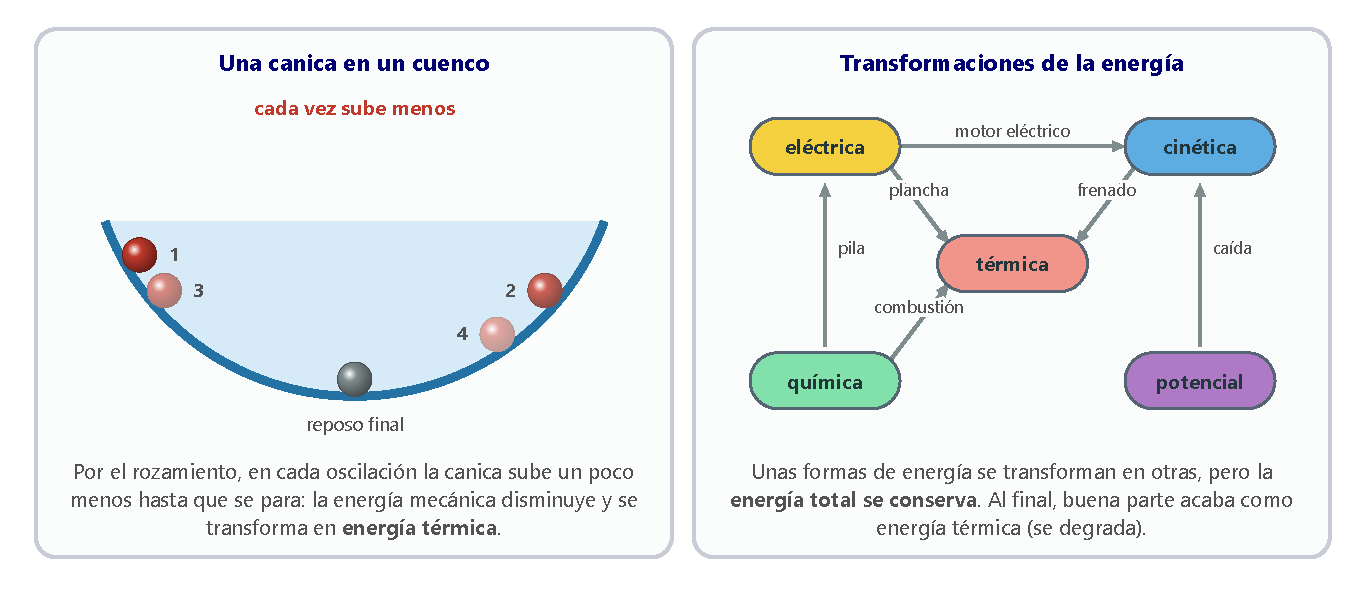
\includegraphics[width=\textwidth]{images/UD11/rozamiento_energia}
    \caption{El rozamiento transforma la energía mecánica en térmica. La energía total se conserva.}
    \label{fig:rozamiento_energia}
\end{figure}

\begin{example}
    ¿Cómo se transforma la energía cuando un futbolista golpea un balón?

    La \textcolor{red}{energía química} de los músculos se transforma en \textcolor{red}{energía cinética} de la pierna y, al golpear, del balón (parte se desprende como calor en los músculos). Mientras rueda, el rozamiento con el césped y el aire transforma su energía cinética en \textcolor{red}{energía térmica}, hasta que se para. La energía no se ha perdido: se ha transformado.
\end{example}

\begin{example}
    Un proyectil de \qty{e-3}{\kg} atraviesa un tablón: entra a \qty{300}{\m\per\s} y sale a \qty{200}{\m\per\s}. a) ¿Qué trabajo ha realizado la fuerza de rozamiento? b) ¿Se ha perdido energía?

    a) \(E_{m,\text{inicial}} = \frac{1}{2} \cdot \num{e-3} \cdot 300^2 = \qty{45}{\joule}\); \(E_{m,\text{final}} = \frac{1}{2} \cdot \num{e-3} \cdot 200^2 = \qty{20}{\joule}\).
    \[ W_{\text{roz}} = E_{m,\text{final}} - E_{m,\text{inicial}} = 20 - 45 = \textcolor{red}{\qty{-25}{\joule}} \]
    b) \textcolor{red}{No}: se ha perdido capacidad de realizar trabajo. Los \qty{25}{\joule} se han transformado en energía térmica (el proyectil y la madera se calientan).
\end{example}

\subsection{¿Una forma de energía se puede transformar en otra?}

Sí: en una plancha, la energía eléctrica se transforma en térmica; cuando un coche frena, la cinética se transforma en térmica; en una pila, la química se transforma en eléctrica; en un motor eléctrico, la eléctrica se transforma en cinética\ldots{} La energía total siempre se conserva, pero en estas transformaciones \textbf{se degrada}, pierde calidad: cualquier forma de energía puede transformarse \emph{íntegramente} en calor, pero el calor \emph{no} puede transformarse íntegramente en otra forma de energía. Por eso tiene sentido hablar de \emph{ahorrar} energía.

\begin{exercise}
    ¿Es correcto decir que en un proceso se ha perdido energía? ¿Y que se ha perdido capacidad para realizar trabajo?
    \begin{solu}
        \textcolor{red}{No} es correcto decir que se ha perdido energía, porque la energía total se conserva. \textcolor{red}{Sí} es correcto decir que se ha perdido capacidad para realizar trabajo: la energía se ha degradado, transformándose en energía térmica.
    \end{solu}
\end{exercise}

\begin{exercise}
    Distingue entre energía mecánica y energía total.
    \begin{solu}
        La \textcolor{red}{energía mecánica} es la suma de las energías cinética y potencial. La \textcolor{red}{energía total} es la suma de todas las formas de energía (mecánica, térmica, química, eléctrica\ldots).
    \end{solu}
\end{exercise}

\begin{exercise}
    Una bola se suelta desde el punto A de una rampa con forma de U y debería llegar al punto B, al otro lado y a la misma altura. ¿Llega hasta B? ¿No se cumple el principio de conservación de la energía mecánica?
    \begin{solu}
        Sin rozamiento llegaría justo hasta B. En la práctica siempre hay \textcolor{red}{rozamiento}, que transforma parte de la energía mecánica en térmica: la bola \textcolor{red}{sube un poco menos} en cada recorrido. La energía mecánica no se conserva, pero la \textcolor{red}{energía total sí}.
    \end{solu}
\end{exercise}

\begin{exercise}
    Describe las transformaciones de energía que se producen en una lámpara.
    \begin{solu}
        La \textcolor{red}{energía eléctrica} se transforma en \textcolor{red}{energía luminosa} y en \textcolor{red}{energía térmica} (la lámpara se calienta).
    \end{solu}
\end{exercise}

\begin{exercise}
    Un coche frena y se detiene. ¿Se ha perdido su energía cinética?
    \begin{solu}
        \textcolor{red}{No}: se ha transformado en \textcolor{red}{energía térmica} en los frenos, los neumáticos y el asfalto.
    \end{solu}
\end{exercise}

\begin{exercise}
    Pon un ejemplo de transformación de: a) energía térmica en mecánica; b) energía eléctrica en mecánica; c) energía eléctrica en química.
    \begin{solu}
        a) Una \textcolor{red}{máquina térmica} (motor de un coche, máquina de vapor). b) Un \textcolor{red}{motor eléctrico} (ventilador, tren eléctrico). c) La \textcolor{red}{electrólisis} o la carga de una batería.
    \end{solu}
\end{exercise}

\subsection*{Actividades de consolidación: conservación de la energía total}

\begin{exercise}
    Enuncia el principio general de conservación de la energía.
    \begin{solu}
        La energía \textcolor{red}{ni se crea ni se destruye, solo se transforma}: en todos los procesos hay intercambios de energía, pero la energía total se mantiene constante.
    \end{solu}
\end{exercise}

\begin{exercise}
    ¿Qué transformaciones de energía tienen lugar en una estufa eléctrica? ¿Y en un aerogenerador?
    \begin{solu}
        En la estufa, la energía \textcolor{red}{eléctrica se transforma en térmica}. En el aerogenerador, la energía \textcolor{red}{cinética del viento se transforma en eléctrica}.
    \end{solu}
\end{exercise}

\begin{exercise}
    Una bala de \qty{15}{\gram} entra a \qty{450}{\m\per\s} en una tabla de \qty{7}{\cm} de espesor. Si la tabla opone una fuerza de rozamiento de \qty{1200}{\newton}, ¿con qué velocidad sale?
    \begin{solu}
        \(E_{c,\text{inicial}} = \frac{1}{2} \cdot \num{0.015} \cdot 450^2 = \qty{1518.75}{\joule}\); \(W_{\text{roz}} = -1200 \cdot \num{0.07} = \qty{-84}{\joule}\).
        \(E_{c,\text{final}} = \num{1518.75} - 84 = \qty{1434.75}{\joule} \Rightarrow v = \sqrt{\dfrac{2 \cdot \num{1434.75}}{\num{0.015}}} = \textcolor{red}{\qty{437}{\m\per\s}}\).
    \end{solu}
\end{exercise}

\begin{exercise}
    ¿Por qué se calienta el cargador de un ordenador portátil o de un móvil cuando está enchufado?
    \begin{solu}
        Porque parte de la \textcolor{red}{energía eléctrica se transforma en energía térmica}: ninguna transformación de energía tiene un rendimiento del \qty{100}{\percent}.
    \end{solu}
\end{exercise}
